%!TEX root =  main.tex
\pagestyle{fancy}
\fancyhf{}
\fancyhead[RE,LO]{\leftmark}
\fancyfoot[CE,CO]{\thepage}
\chapter{Introduction}\label{chapter:Intro}
%
Various software systems has changed the way people communicate, learn and run businesses, and interconnected computing devices has numerous positive applications in everyday life. Over the past decade, computation and data volumes have increased significantly~\cite{ChiangZ16}. Augmented reality, online gaming, face recognition, autonomous vehicles, or the Internet of Things (IoT) applications produce huge volumes of data. Workloads like those require latency below a few tens of milliseconds~\cite{ChiangZ16}. These requirements are outside what a centralized model like the cloud computing can offer~\cite{ChiangZ16}. Even small problems can contribute to large downtime of applications and servies people are depending on. Recent example is yet another outage that happend in Amazon Web Services (AWS), and as a result a large amount of internet become unavaleble.

The aim of this thesis is to provide formal models uppon which we implement distributed system for oragnizing cloud-like geo-distributed environments for users or CC providers to utilize, in order to minimize downtime of critical services. The whole system can be looked as a micro-clouds or pre-processing layer sending only important data to the cloud minimizing cost for users, and ensuring avelability of CC services.

In this section, we are going to give an overview of the topics, that are of significant importance for the rest of the thesis, since it is heavely based on these topis. We start by describing the general problem area that our work addresses in Section~\ref{sec:problem_area}. Sections~\ref{sec:distributed_systems} and \ref{sec:distributed_computing} describe the theoretical background behind the problem, where we examine distributed systems (DS) and distributed computing (DC), focusing on design details, communication patters and organizational structure. In Section~\ref{sec:similar_models} we describe similar models that might be source of confusion, and how they are differnet than DS or DC and how some concepts can fit in the bigger picture. Section~\ref{sec:deployment} describe different architecture and application model and how deployment can be done in large DS. In Section~\ref{sec:virtualization_techniques} we describe different virtualization methods that are used in CC for system and/or applications. In section~\ref{sec:concurency_parallelism} we describe difference between concurency and parallelism and introduce actor system, that will be used latter on in the thesis. In Section~\ref{sec:problem_statement}, we specify the exact problem that our work addresses and describe our hypothesis and research goals in Section~\ref{sec:research_hyphotesis_and_golas}. Section~\ref{sec:structure_of_thesis} present the structure of the thesis.
%
%
%
\section{Problem area}\label{sec:problem_area}
%
Cloud centralized architecture with enormous data-centers (DCs) capacities creates an effective economy of scale to lower administration cost~\cite{BariBEGPRZZ13}. However, when such a  system grows to its limits, centralization brings more problems than solutions~\cite{GunawiHSLSAE16, LopezMEDHIBFR15}. Despite all the CC benefits, applications and services face a serious degradation over time, due to the high bandwidth and latency~\cite{KarimIWGSYO16}. This can have a huge consequence on the business and potentially human lives as well. Organizations use cloud services to avoid huge investments~\cite{MonsalveCC18}, like creating and maintaining their own DCs. They consume resources created by others~\cite{Satyanarayanan17} and pay for usage time -- a pay as you go model.

Data is required to be moved to the cloud from data sources, which introduces a high latency in the system~\cite{HossainRH18}. For example, Boeing 787s generates half a terabyte of data per single flight, while a self-driving car generates two petabytes of data per single drive. Bandwidth is not large enough to support such requirements~\cite{CaoZS18}. Data transfer is not the only problem: applications like self-driving cars, delivery drones, or power balancing in electric grids require real-time processing for proper decision making \cite{CaoZS18}. We might face serious issues if a cloud service becomes unavailable due to denial-of-service attack, network, or cloud failure~\cite{GunawiHSLSAE16}.

To overcome cloud latency, research led to new computing areas, and model in which computing and storage utilities are in proximity to data sources~\cite{Satyanarayanan17}. The cloud is enhanced with new ideas for future generation applications~\cite{NingLSY20}. 
%
%
%
\section{Distributed systems}\label{sec:distributed_systems}
%
There are various definitions of DS, but we can think of DS as a systems where multiple entities can comunicate to one another in some way, but at the same time, they are able to performing some operations. 

In~\cite{SteenT16, 0019513} Tanenbaum et al. give two interesting assumption about DS:

\begin{enumerate}[start=1,label={(\bfseries \arabic*)}]
	\item  \say{A computing element, which we will generally refer to as a node, can be either a hardware device or a software process}.
	\item \say{A second element is that users (be they people or applications) believe they are dealing with a single system. This means that one way or another the autonomous nodes need to collaborate}.\label{ds:asumption_2}
\end{enumerate}

\noindent
These two assamptions are usefull and powefull, when talking about DS. As such, in this thesis we will adopt and use them rigorously.

Three significant characteristics of distributed systems are~\cite{0019513}: 

\begin{enumerate}[start=1,label={(\bfseries \arabic*)}]
	\item \textbf{concurrency of components}, referst to ability of the DS that multiple activities are executed at the same time. These activities takes place on multiple nodes that are part of a DS.
	\item \textbf{independent failure of components}, this property refers to a nasty feature of DS that nodes fail independently. Thy can fail at the same time as well, but they usually fail independently for numerus reasons.
	\item \textbf{lack of a global clock}, this is a consequence of dealing with independent nodes. Each node have its own notion of time, and such we cannot assume that there is something like a global clock.
\end{enumerate} 

In~\cite{SteenT16} authors give formal definition \say{distributed system is a collection of autonomous computing elements that appears to its users as a single coherent system}.

When talking about DS, we usually think about computing systems that are connected via network or over the internet. But DS are not exclusiv to domain of cumputer science. They existed before computers started to enrich almost every aspect of human life. DS have been used in varios different domains such as: \textbf{telecommunication networks}, \textbf{aircraft control systems}, \textbf{industrial control systems} etc. DS are used anywhere where amout of users are growing rapidly, so that single entity can't reponse to users demands in (near) real-time.

Distributed systems (in computer science) are consists of various algorithms, techniques and trade-offs to create an illusion that set of nodes act as one. DS algorithms may include: $(1)$ replication, $(2)$ consensus, $(3)$ communication, $(4)$ storage, $(5)$ processing, $(6)$ membership etc.

DS are hard to immplement because of their nature. James Gosling and Peter Deutsch both fellows at Sun Microsystems at the time crated list of problems for network applicatoins know as \textit{8 fallacies of Distributed Systems}:\label{enum:fallacies}

\begin{enumerate}[start=1,label={(\bfseries \arabic*)}]\label{ds:8_fallacies}
	\item \textbf{The network is reliable}; there will always be something that go wrong with the network --- power failure, a cut cable, environment disasters etc.
	\item \textbf{Latency is zero}; localy latency is not an issue, but it deteriorates very quickly when you move to the internet and CC scenarios.
	\item \textbf{Bandwidth is infinite}; even though bandwidth is constantly getting better and better, the amount of data we try to push through it rise as well.
	\item \textbf{The network is secure};  Internet attack trends are showing growth, and this becomes problem even more in public CC.
	\item \textbf{Topology doesn't change}; network topology is usually out of user control, and network topology changes sonstantly for numerous of reasons --- added or removed new devices, servers, breaks, outages etc.
	\item \textbf{There is one administrator}; nowdays there are numerous of administratos for web servers, databases, cache and so one, but also company collaborates with other copanies or CC provider.
	\item \textbf{Transport cost is zero}; we have to serialize information and send data over the wire, which takes resources and adds to the total latency. Problem here is not just latency,but that information serialization takes time and resources.
	\item \textbf{The network is homogeneous}; today, homogeneous network is the exception, rather then a rule. We have different servers, systems, clients that interacts. The implication of this is that we have to assume interoperability between these systems sooner or later but we must be aware of it. We might also have some  proprietary protocols that might also take time to send on and they may stay without support, so we should avoid them.
\end{enumerate}

These fallacies are intruduced over the dacade ago, and more than four decades since we started building DS, but the characteristics and underlying problems remains pretty the same. It is interesting fact that designers, architects still asume that technology solves everything. This is not the case in DS, and these fallacies should not be forgoten. Because of these problems, DS are hard to implement corectly and they are hard to test and maintain.
%
%
\subsection{Scalability}\label{sec:scalability}
%
Scalability is the property of a system to handle a growing amount of work by adding resources to the system~\cite{Bondi00}. When talking about computer systems scalability can be represented in two flavors:

\begin{itemize}
	\item \textbf{Scaling vertically} means upgradeing the hardware that computer systems are running on. Vertical scaling can increase performance to what latest hardware can offer, and here we are limited by the laws of phisics and Moor's law \cite{Gustafson2011}. Tipical example that require this type of scaleing is relation dataase server. These capabilities are insufficient for moderate to big workloads.
	\item \textbf{Scaling horizontally} means that we scale our system by keep adding more and more computers, rather than upgrading the hardware of a single one. With this apporouch we are (almost) limitless how much we can scale. Whenever performance degrades we can simply add more computers (or nodes). These nodes are not required to be some high-end machines.
\end{itemize}

Table~\ref{tab:table1} summarize differences between horizontall and verticall scaling.

\begin{table}[h!]
	\begin{center}
		\begin{tabular}{l|l|l}
			\textbf{Feature} & \textbf{Scaling vertically} & \textbf{Scaling horizontally}\\
			\hline
			\textbf{Scaling} & Limited & Unlimited \\
			\textbf{Managment} & Easy & Comlex\\
			\textbf{Investments} & Expensive & Afordable \\
		\end{tabular}
	\end{center}
	\vspace{-0.5cm}
	\caption{Differences between horizontall and verticall scaling.}
	\label{tab:table1}
\end{table}

Scaling horizontally is a preferable way for scaling DS, not because we can scale easier, or because it is significantly cheaper than vertical scaling after a certain threshold~\cite{Bondi00} but because this approuch comes with few more benefits that are esspecially important when talking about large-scale DS. Adding more nodes gives us two important properties: 

\begin{itemize}
	\item \textbf{Fault tolerance} means that applications running on multiple places at the same time, are not bound to the fail of a node, cluster or even DCs. As long as there is a copy of application running somewhere, user will get response back. As a consequence of runnin multiple copies of a service and on multiple places, we have that service is more \textbf{avalible}, that running on a single node no metter how high-end that node is. Eventually all nodes are going to break, and if we have multiple copies of the same service we have more resilient and more avalible system to serve user requests.
	\item \textbf{Low latency} refers to the idea that the world is limited by the speed of light. If a node running application is too far away, user will wait too long for the response to get back. If same application is running on multiple places, user request will hit node that is closest to the user.
\end{itemize}

But despite all the obvious benefits, for a DS to work properly, we need the write software in such a way that is able to run on multiple nodes, as well as that accept \textbf{failure} and deal with it. This turns out to be not an easy task.

For example users need to be aware when using DS, is related to distributed data storage systems. Storage implementations that relys on vertical scaling to ensure scalability and faulte tolerance, have one nasty feature. 

This nasty feature is represented in theorem called \textbf{CAP theorem} presented by Eric Brewer~\cite{Brewer2000}, and proven after insepction by Bilbert et a.~\cite{GilbertL02}. The CAP theorem states that it is impossible for a distributed data store to simultaneously provide more than two out of three guarantees shown in Figure~\ref{fig:fig17}.

\begin{figure}[H]
	\begin{center}
		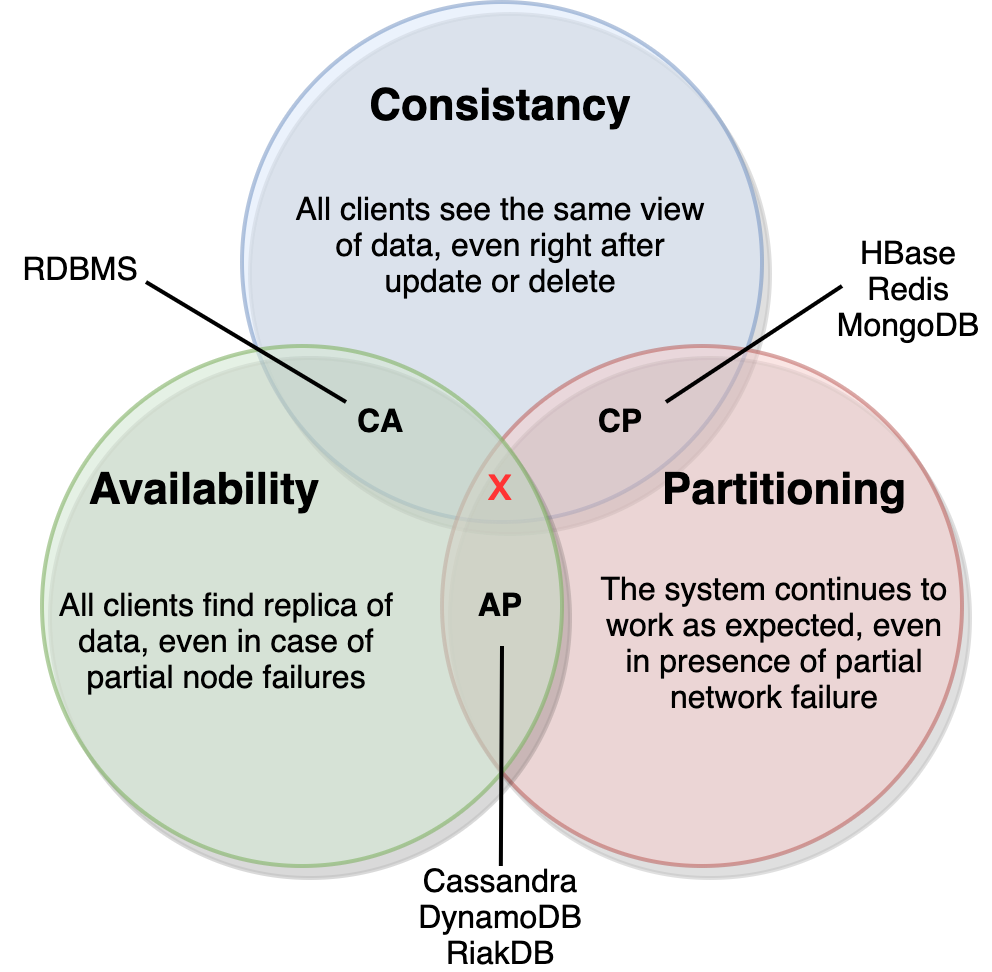
\includegraphics[scale=0.9]{images/Figure17.png}
	\end{center}
	\vspace{-0.6cm}
	\caption{Difference between cloud options and on-premises solution.}
	\label{fig:fig17}
\end{figure}

\begin{enumerate} [start=1,label={(\bfseries \arabic*)}]
	\item \textbf{C}onsistency, which means that all clients will see the same data at the same time, no matter which node they are connected to. Clients my not be connected to the same node since data could be replicated on many nodes in different locations.
	\item \textbf{A}vailability, which means that any client issued a request will get response back, even if one or nodes are down. DS will not interprate this situation as an exception or error. Availability is represented in percentage, and it describe how much downtime is allowed per year, This can be calculated using formula:\\ 
	
	\begin{equation}\label{eq:Availability}
		Availability = \frac{uptime}{ (uptime + downtime)}
	\end{equation}
	\myequations{Availability percentage formula}
	Industry is using measureing avelability in \say{class of nines}. Availability class is the number of leading nines in the availability figure for a system or module~\cite{GrayS91}. This metric relates to the amount of time (per year) that a service is up and running. Table~\ref{tab:table7} show different classes of nine and their availability and unavailability in minutes per year (\textbf{min/year}) for some examples~\cite{GrayS91}.
	
	\begin{table}[h!]
		\begin{center}
			\begin{tabular}{l|l|l}
				\textbf{Type} & \textbf{Availability} & \textbf{Unavailability} \\
				\hline
				\textbf{Unmanaged} & 90\% & 50,000 \\
				\textbf{Managed} & 99\% & 5,000 \\
				\textbf{Well-managed} & 99.9\% & 500 \\
				\textbf{Well-managed} & 99.9\% & 500 \\
				\textbf{Fault-tolerant} & 99.99\% & 50 \\
				\textbf{High-availability} & 99.999\% & 5 \\
				\textbf{Very-high-availability} & 99.9999\% & 0.5 \\
			\end{tabular}
		\end{center}
		\vspace{-0.5cm}
		\caption{Downtime for different classes of nines.}
		\label{tab:table7}
	\end{table}
	
	We can calculate availability class if we have system availability $A$, the system's availability class is define as~\cite{GrayS91}: 
	
	\begin{equation} 
		e^{\log_{10} \frac{1}{ (1 - A)}} 
	\end{equation}
	\myequations{Availability class formula.}
	It is important to notice that even a 99\% available system gives almost four days of downtime in a year, which is unacceptable for services like Facebook, Google, AWS etc. And when service is down, companies are loosing customers.
	\item \textbf{P}artition tolerance, which means that the cluster must continue to work despite any number of communication breakdowns between nodes in the system. It is important to state that in a distributed system, partitions can’t be avoided.
\end{enumerate}

Years after CAP theorem inception, Shapiro et al. prove that we can alleviate CAP theorem problems, but only in some cases, and offers \textbf{Strong Eventual Consistency (SEC) model}~\cite{ShapiroPBZ11}. They prove that if we can represent our data structure to be: \label{crdts}

\begin{itemize}
	\item \textbf{Commutative} $a*b = b*a$ \myequations{Commutative formula.}
	\item \textbf{Associative} $(a*b)*c = a*(b*c)$ \myequations{Associative formula.}
	\item \textbf{Idempotent} $(a * a) = a$ \myequations{Idempotent formula.}
\end{itemize}

\noindent
where $*$ is a binary operation, for example: $max$, $union$, $or$ we can rely on SEC properties,
%
%
\subsection{Cloud computing}\label{sec:cloud_computing}
%
We can define cloud computing (CC) like aggregation of computing resources as a utility, and software as a service~\cite{Vogels}. Hardware and software in big DCs provide services for user consumption over the internet~\cite{AboveTheCloud}. Resources like CPU, GPU, storage, and network are utilities and can be used as well as released on-demand~\cite{ZhangCB10}. The key strength of the CC are offered services~\cite{Vogels}. 

The traditional CC model provides enormous computing and storage resources elastically, to support the various applications needs. This property refers to the cloud ability to allow services, allocation of additional resources, or release unused ones to match the application workloads on-demand~\cite{AssuncaoVB18}. Services usually fall in one of three main categories: 

\begin{itemize}
	\item \textbf{Infrastructure as a service (IaaS)} allows businesses to purchase resources on-demand and as-needed instead of bying and manageing hardware themself.
	\item \textbf{Platform as a service (PaaS)} delivers a framework for developers to create, maintain and manage their applications. All resources are managed by the enterprise or a third-party vendor.
	\item \textbf{Software as a service (SaaS)} deliver applications over the internet to its users. These applications are managed by a third-party vendor, .
\end{itemize}

Figure~\ref{fig:fig1} show difference in control and management of resources between different cloud options and on-premises solution.

\begin{figure}[H]
	\begin{center}
		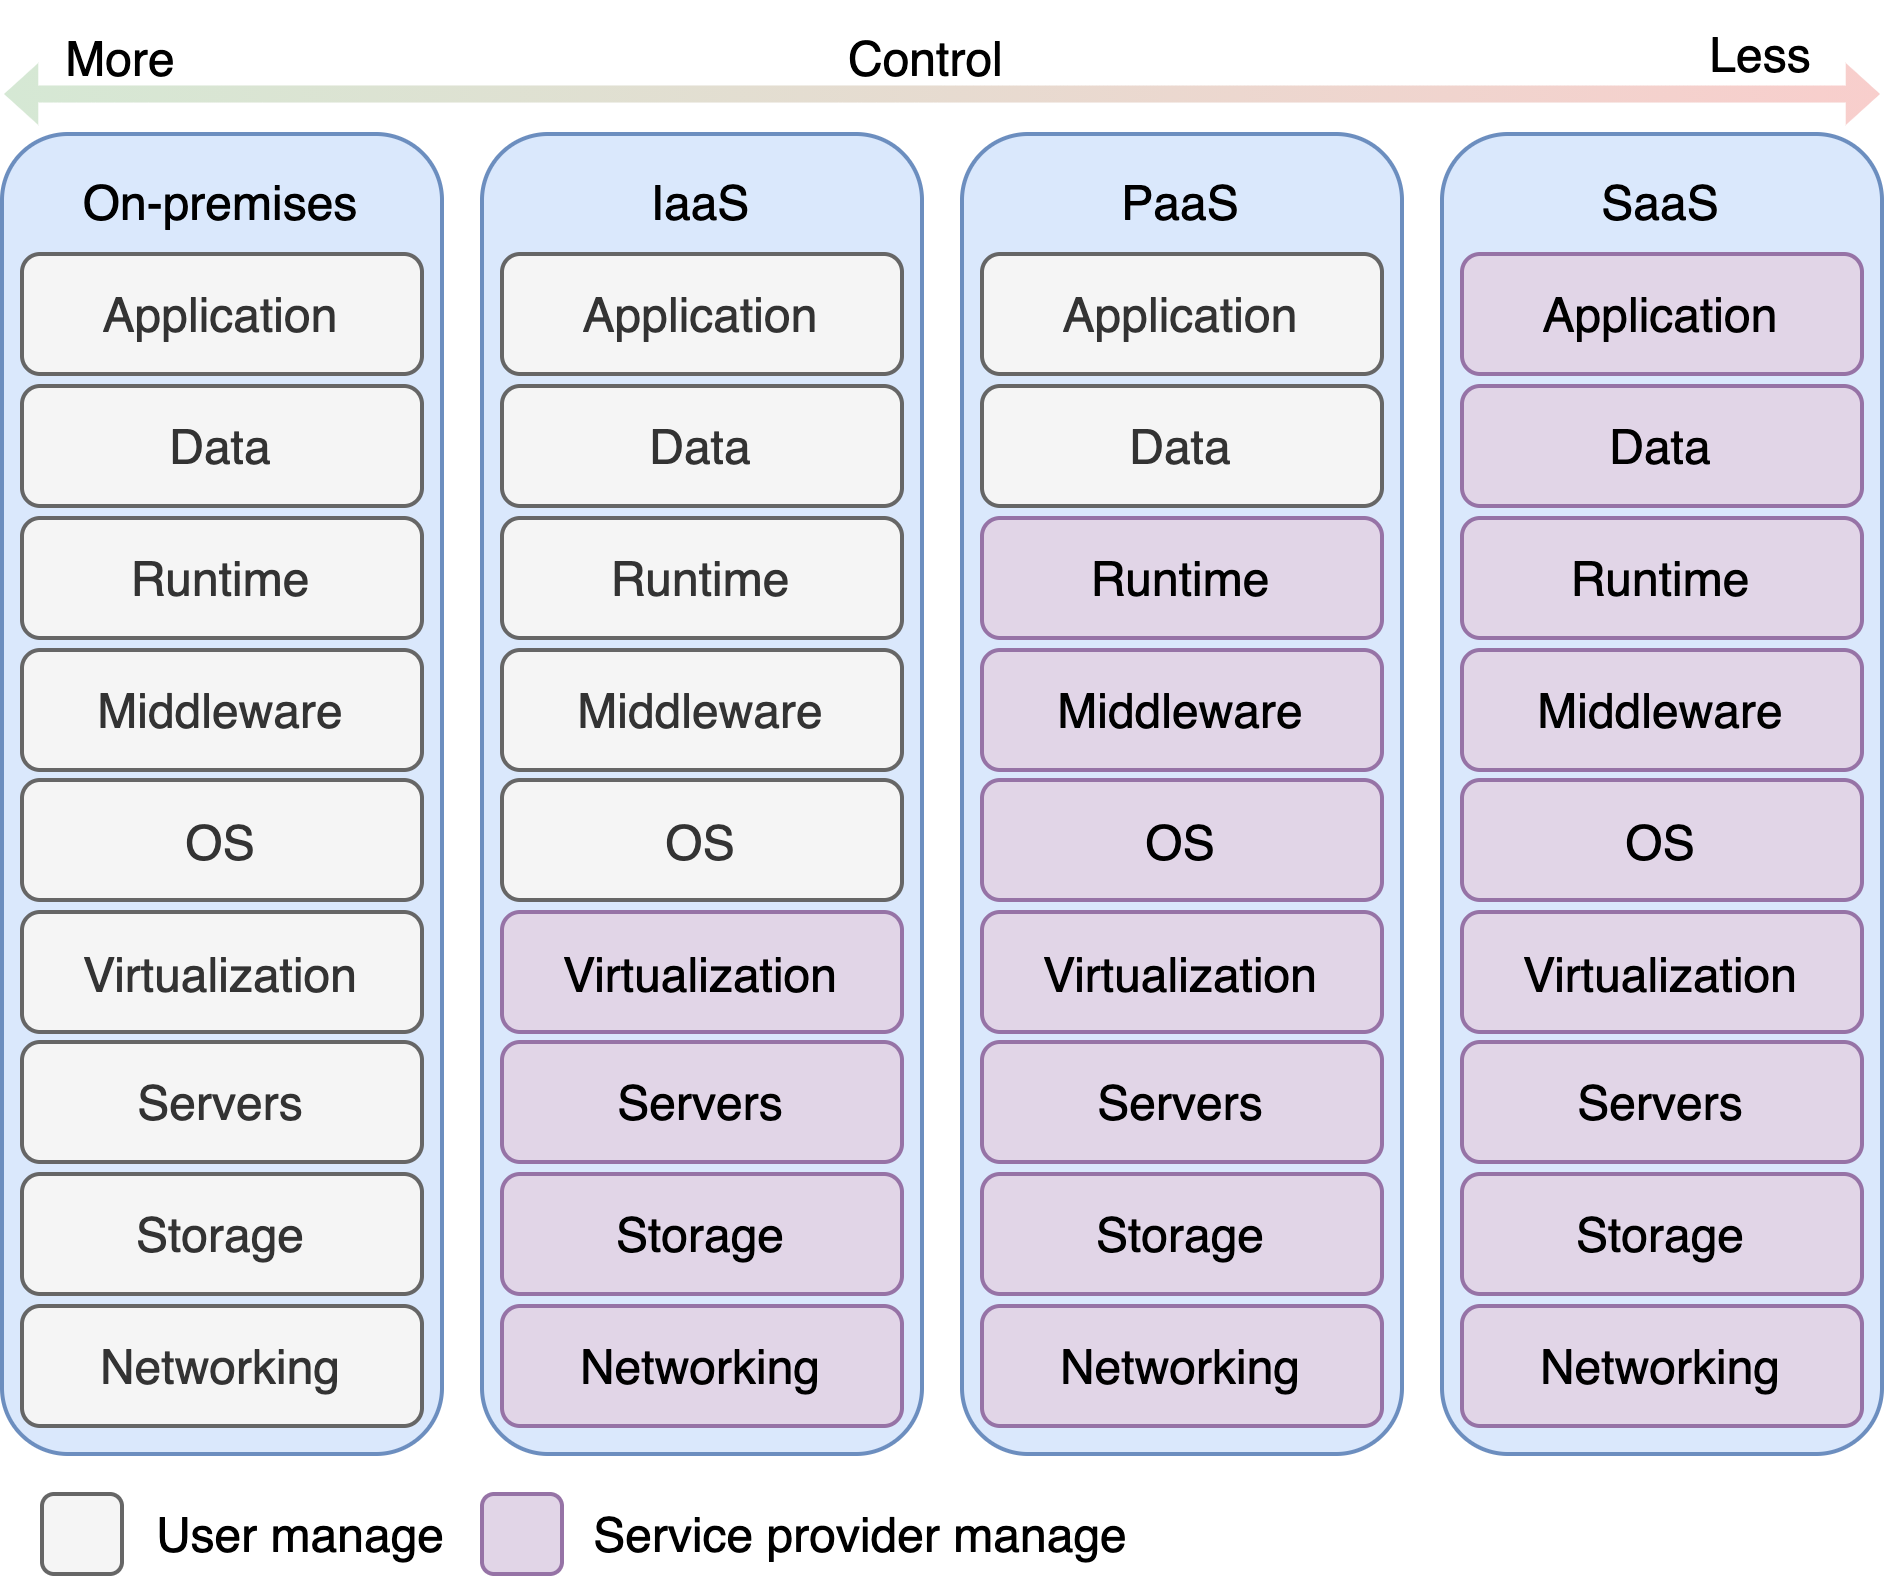
\includegraphics[scale=0.9]{images/Figure1.png}
	\end{center}
	\vspace{-0.6cm}
	\caption{Difference between cloud options and on-premises solution.}
	\label{fig:fig1}
\end{figure}

The user can choose a single solution, or combine more of them if such a thing is required depending on preferences and needs.

By the ownership, CC can be categorized into three categories:

\begin{itemize}
	\item \textbf{Public cloud} is type where CC is delivered over the internet, and shared across many many organizations and users. In this type of the CC, architecture is built and maintained by others. Users and organizations pay for what they use. Examples include: AWS EC2, Google App Engine, Microsoft Azure etc.
	\item \textbf{Private cloud} is type where CC is dedicated only to a single organization. In this type of the CC, architecture is built by organization who may offer their solution or services to the users or other organizations. These services are in domain what the organization does, and that organization is in charge of maintanance. Examples include VMWare, XEN, KVM etc.
	\item \textbf{Hybrid cloud} is such environment that uses both public and private clouds. Examples include: IBM, HP, VMWare vCloud etc.
\end{itemize}

Table~\ref{tab:table4} show comparison of public, private and hybrid cloud capabilities.

\begin{table}[h!]
	\begin{center}
		\begin{tabular}{l|l|l|l}
			\textbf{Capabilities} & \textbf{Public cloud} & \textbf{Private cloud} & \textbf{Hybrid cloud}\\
			\hline
			\textbf{Data control} & IT enterprise & Service Provider & Both \\
			\textbf{Cost} & Low & High & Moderate \\
			\textbf{Data security} & Low & High & Moderate \\
			\textbf{Service levels} & IT specific & Provider specific & Aggregate \\
			\textbf{Scalability} & Very high & Limited & Very high \\	
			\textbf{Reliability} & Moderate & Very high & Medium/High\\	
			\textbf{Performance} & Low/Medium & Good & Good \\
\end{tabular}
	\end{center}
	\vspace{-0.5cm}
	\caption{Comparison of public, private and hybrid cloud capabilities.}
	\label{tab:table4}
\end{table}

In the rest of the thesis, if not stated differently when CC term is used it denotes public cloud.

CC has been the dominating tool in the past decade in various applications~\cite{Satyanarayanan17}. It is changing, evolving, and offering new types of services. Resources such as container as a service (CaaS), database as a service (DBaaS)~\cite{Peter} are newly introduced. The CC model gives us a few benefits. Centralization relies on the economy of scale to lower the cost of administration of big DCs. Organizations using cloud services avoid huge investments. Like creating and maintaining their own DCs. They consume resources usually created by others~\cite{Satyanarayanan17} and pay for usage time -- a pay as you go model. 

But centralization give us few really hard problems to solve. As already stated in section~\ref{sec:problem_area} data is required to be moved to the cloud from data sources, which introduces a high latency in the system~\cite{HossainRH18}. 

There are few notable attempts to help data ingestion into the cloud. Remote Direct Memory Access (RDMA) protocol makes it possible to read data directly from the memory of one computer and write that data directly to the memory of another. This is done by using \textit{specialized hardware} interface cards and switches and software as well, and operations like read, write, send, receive etc. do not go through CPU. With this caracteristivs, RDMA have low latencies and overhead, and as such reach better throughputs~\cite{CohenTKCKRCDG09}. This new hardware may not be cheap, and not evey CC provider use them for every use-case. And this may not be enough, esspecially with ever growing amount of IoT devices and services.

Over the years there are more as a service options avalible, forming \textbf{everything as a service (XaaS)} model~\cite{DuanFZSNH15}. This model propose that any hardware or software resource can be ofered as a service to the users over the internet.

Table~\ref{tab:table2} shows common examples of SaaS, PaaS, and IaaS applications.

\begin{table}[h!]
	\begin{center}
		\begin{tabular}{l|l}
			\textbf{Platform type} & \textbf{Common Examples}\\
			\hline
			\textbf{IaaS} & AWS, Microsoft Azure, Google Compute Engine \\
			\textbf{PaaS} & AWS Elastic Beanstalk, Azure, App Engine \\
			\textbf{SaaS} & Gmail, Dropbox, Salesforce, GoToMeeting \\
		\end{tabular}
	\end{center}
	\vspace{-0.5cm}
	\caption{Common examples of SaaS, PaaS, and IaaS.}
	\label{tab:table2}
\end{table}

CC is giving a user an illusion that he is using single machine, while the backgroud implementaion is fairly complicated and consists of various elements that are composed of countles machines. CC is tipical example of horizontally scalable system presented in~\ref{sec:scalability}
%
%
\subsection{Membership protocol}\label{sec:memership_protocol}
%
A the start of this section we introduced DS, and we present two interesting assumptions by Tanenbaum et al.~\cite{SteenT16, 0019513}. If we take one more look at the~\ref{ds:asumption_2} assumption, we will see that user of the DS whether they are users or applications perceive DS as a single element. Inside this single elements nodes need to colaborate, so that they are albe to do various kinds of tasks.

Most basic of all these tasks, is that nodes needs to know which group they belog to, and who are their peers in the group they will colaborate with. This might sound as a trivial idea, but when we include 8 fallacies of the DS~\ref{ds:8_fallacies} into the equation, things start to be not so trivial, after all. In the setup where nodes are connected over the local network or internet, and they need to communicate things will go wrong for various reasons.

To resolve the problem that nodes need to know who are their group peers, a membership protocols come to help. These protocols needs to ensures that each process of one group updates his local list of \textbf{non-faulty} members of the group, and when a new process joins or leaves the group, local list for every process needs to be updated. This is the most basic idea behind membership protocols.

Processes in the group, or nodes in a group will ping each other in different ways, and using different strategies to figure out which nodes are dead and which are alive. There are few existing algorithms that does this job, and they are (usually) based on the way epidemics spread or how gossip is spreaded in population. Because of this feature these algorithms are usually called \textit{Gossip} style protocols.

Every membership protocol have some properties that will ensure efficiency and scalability:

\begin{enumerate}[start=1,label={(\bfseries \arabic*)}] \label{ds:features}
	\item \textbf{Completeness}, this property must ensure that every failure in the system is detected.
	\item \textbf{Accuracy}, in ideal world, there should be no mistakes when detecting failures. But In real life scenario, we need to reduce false positives as much as we can.
	\item \textbf{Failure detection speed}, all failures needs to be tected as fast as possible, in order to remove the node from the group and reschedule the tasks from dead node to alive ones.
	\item \textbf{Scale}, with this property we must ensure that the network load that is generated should be distributed equally between all processes in the group.
\end{enumerate}

Easiest idea to implement this protocol would be \textbf{heartbeating} technique where process $P_i$ will send heartbeat message to all his peers in the group or \textbf{multicast}. After some time if process $P_j$ did not receive heartbeat message from $P_i$, it will mark him as faild. This idea is easy to understand, and implement but downsides are that his process is not really \textbf{scalable}, esspecially for large groups, and this will introduce huge network traffic.

To resolve this problem, Das et al.~\cite{DasGM02} introduced \textbf{S}calable \textbf{W}eakly-consistent \textbf{I}nfection-style Process Group \textbf{M}embership protocol, or \textbf{SWIM} for short. This protocol divides the membership problem into two parts:

\begin{enumerate}[start=1,label={(\bfseries \arabic*)}]
	\item \textbf{Failure detection}, this component works so that one node will select random node in the group, and it will send him $ping$ message, expecting $ack$ message in return --- \textbf{direct ping}. If such message is not received, he will pick $n$ nodes to probe through a $ping-req$ message --- \textbf{indirect ping}. If this fail, node will be marked as $suspected$, and it will be marked as $dead$ after some timeout. If node get alive, he will ping some other node and he will get back into the group. Figure~\ref{fig:fig15} show message passing in \textbf{direct} $(left)$, and \textbf{indirect} $(right)$ ping in SWIM protocol.
	\item \textbf{Information dissemination}, with previous strategy, we can disseminate information by \textbf{piggybacking} the data on multiple messages ($ping$, $ping-req$ and $ack$), and avoid using the multicast solution.
\end{enumerate}

\begin{figure}[H]
	\begin{center}
		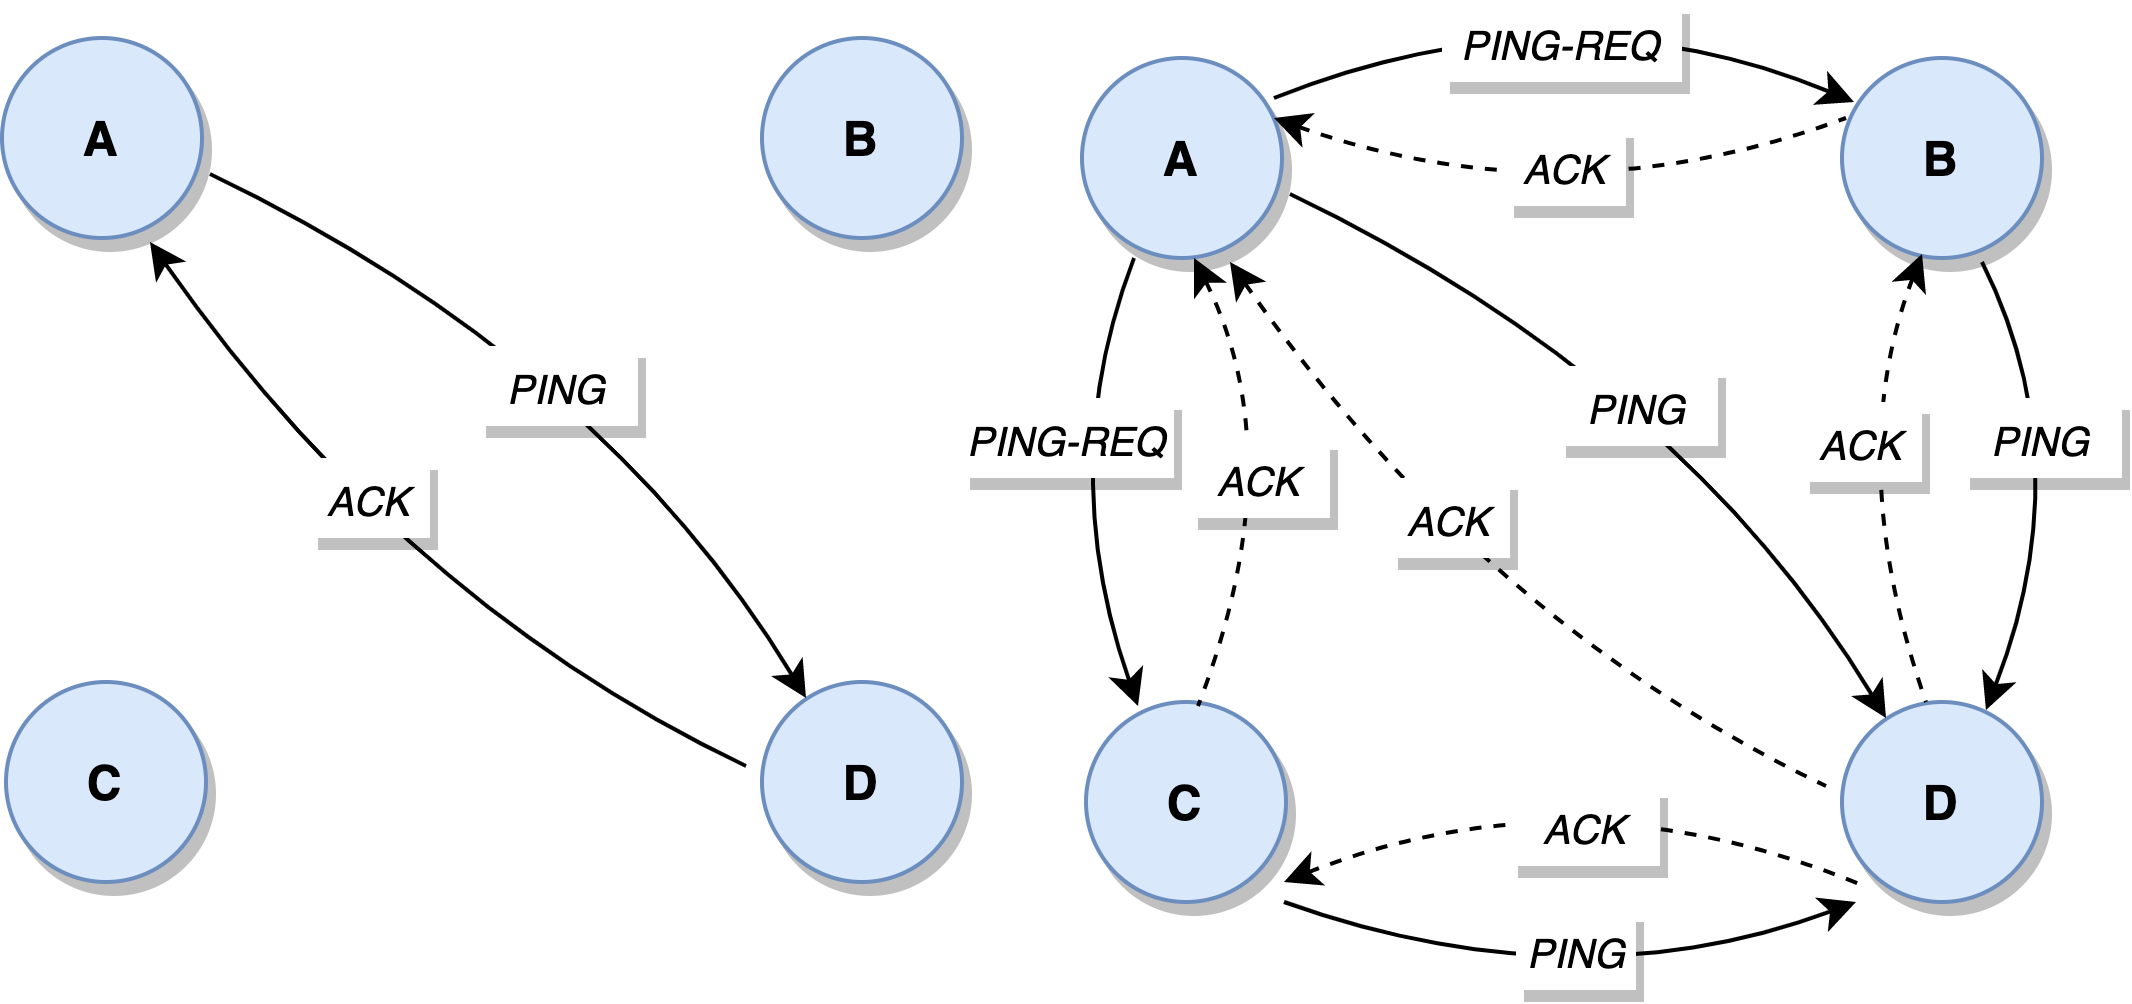
\includegraphics[scale=0.7]{images/Figure15.png}
	\end{center}
	\vspace{-0.6cm}
	\caption{Direct and indirect ping in SWIM protocol.}
	\label{fig:fig15}
\end{figure}

Over the years, reserchers foud ways to improve the protocol for example Dadgar et al. present Lifeguard protocol~\cite{DadgarPC18} for more
acccurate failure detection, and there are other implementations to fine tune the SWIM, but base idea is still there. Today SWIM or SWIM-like protocols are standard membership procol whenever we are doing some node clustering.
%
%
\subsection{Mobile computing}\label{sec:mobile_computing}
%
Mobile cloud computing (MCC), was the first idea that introduced task offloading~\cite{FernandoLR13, LinLJL19}. Heavy computation remains in the cloud. Mobile devices run small client software and interact with the cloud, over the internet using his resources. 

The main problem with MCC is that the cloud is usually far away from end devices. That leads to high latency and bad quality of experience (QoE)~\cite{LinLJL19}. Especially for latency-sensitive applications. Even though MCC is not that much different from the standard cloud model. We had moved a small number of tasks from the cloud. Thus opening the door for future models.

To overcome cloud latency and MCC problems, research led to new computing areas like edge computing (EC). EC is a model in which computing and storage utilities are in proximity to data sources~\cite{Satyanarayanan17}. The cloud is enhanced with new ideas for future generation applications~\cite{NingLSY20}. 

Over the years, designs like fog~\cite{BonomiMNZ14}, cloudlets~\cite{MonsalveCC18}, and mobile edge computing (MEC)~\cite{WangZZWYW17} emerged. In this thesis, we refer to all these models as edge nodes. They all use the concept of data and computation offloading from the cloud closer to the ground~\cite{KhuneP19}, while heavy computation remains in the cloud because of resource availability~\cite{NingLSY20}. 

EC models introduce small-scale servers that operate between data sources and the cloud. Typically, they have much less capabilities compared to the cloud counterparts~\cite{ChenHLLW15}. These servers can be spread in base stations~\cite{WangZZWYW17}, coffee shops, or over geographic regions to avoid latency as well as huge bandwidth~\cite{MonsalveCC18}. They can serve as firewalls~\cite{SatyanarayananK19} and pre-processing tier, while users get a unique ability to dynamically and selectively control the information sent to the cloud.
%
%
\section{Distributed computing}\label{sec:distributed_computing}
%
DC can be defined as the use of a DS to solve one large problem by breaking it down into several smaller parts, where each part is computed in the individual node of the DS and coordinatio is done by passing messages to one another~\cite{0019513}. Computer programs that use this strategy and runs on DS are called \textbf{distributed programs} \cite{Vera16, andrews2000foundations}. 

Similar to CC in Section~\ref{sec:cloud_computing}, to a normal user, DC systems appear as a single system similar to one he use every day on his personal computer. DC share same fallacies to DS presented in~\ref{sec:distributed_systems}.
%
%
\subsection{Big Data}\label{sec:big_data}
%
Tearm big data means that the data is unable to be handled, processed or loaded into a single machine~\cite{FisherDCD12}. That menas that traditional data mining methods or data analytics tools developed for a centralized processing  may not be able to be applied directly to big data~\cite{Tsai2015}. 

New tools and methos that are developed are relying on DS and one specific feature \textbf{data locality}~\label{ds:data_locality}. Data locality can be described as a process of moving the computation closer to the data, instead of moving large data to computation~\cite{GuoFZ12}. This simple idea, minimizes network congestion and increases the overall throughput of the system.

In~\ref{sec:problem_area} we already give two examples how huge generated data could be, and when we incude other IoT sensors and devices these numbers will just keep getting bigger~\cite{SarigiannidisLR20}.

On contrary to relational databases that mostly deal with structured data, big data is dealing with various kinds of data~\cite{FisherDCD12, Tsai2015, GuoFZ12}:

\begin{itemize}
	\item \textbf{Structured} data is kind of data that have some fixed structure and format. Tipical example of this is data stored inside table of some database. organizations susully have no huge problem extracting some kind of value out of the data.
	\item \textbf{Unstructured} data is kind of data where wo do not have any kind of structure at all. These data sources are heterogeneous and may containing a combination of simple text files, images, videos etc. This type of data is usully in raw format, and organizations have hard time to derive value out.
	\item \textbf{Semi-structured} data is kind of data that can contain both previously mentioned types of data. Example of this type of data is XML files.
\end{itemize}

Along it's share size, big data have other instantly recognizable features called \textbf{V's} of big data~\cite{PatgiriA16}. Name is derived from starting letters from the other features that are describing big data. Image~\ref{fig:fig3} show 6 V's comonly used to represent the big data.

\begin{figure}[H]
	\begin{center}
		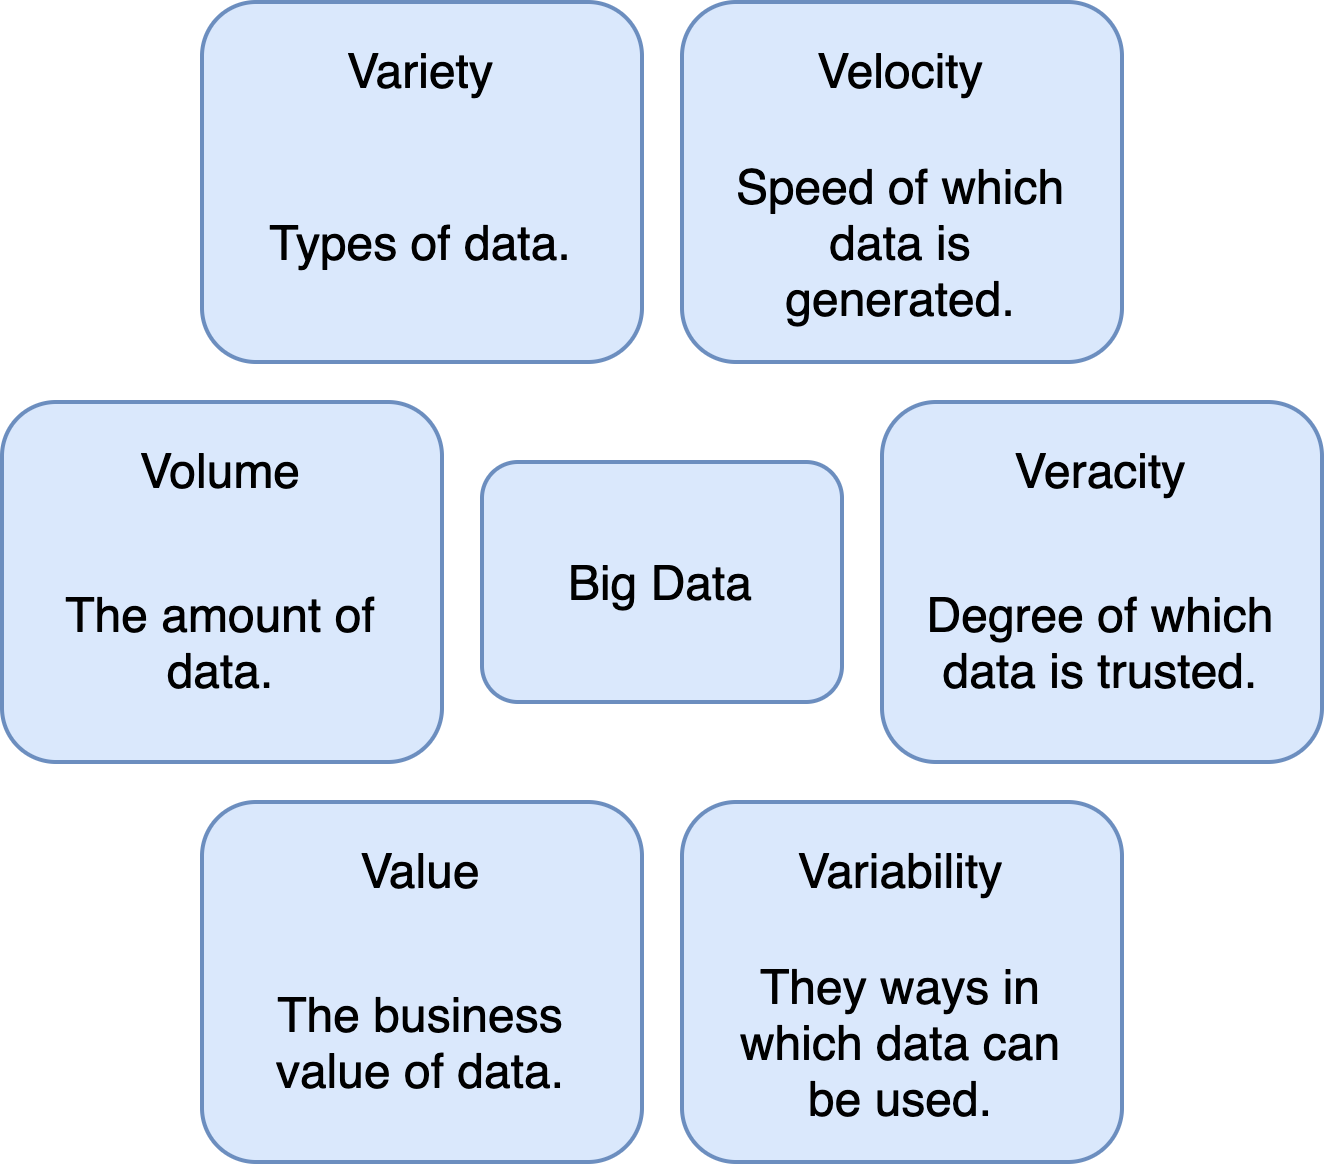
\includegraphics[scale=0.7]{images/Figure3.png}
	\end{center}
	\vspace{-0.6cm}
	\caption{V's of Big Data.}
	\label{fig:fig3}
\end{figure}

Processing in big data systems can be represented as~\cite{phdthesis, KiranMMDB15}:

\begin{itemize}
	\item \textbf{Batch processing} represents data prcessing technique that is done on huge quantity of the stored data. This type of prcessing is usually slow and requure time.
	\item \textbf{Stream processing} represents data processing technique that is done as data get into the system. This type of processing is usually done on smaller quantity of the data \textbf{at the time}, and it is faster.
	\item \textbf{Lambda architectures} represents processing technique where stream processing and handling of massive data volumes in batch are combined in a uniform manner, reducing costs in the process~\cite{KiranMMDB15}.
\end{itemize}

Big data systems, are not processing and value extracting systems. Big data systems can be separated in few categories: $(1)$ data storage, $(2)$, data ingestion $(3)$, data processing and analytics. All these system aids to properly analyze ever growing requirements~\cite{RaoMBG19},

Dispite promise that big data offers to derive value out of the collected data, this task is not easy to do and requre properly set up system filtering and removeing data that contains no value. To aid this idea, data could be filtered and little bit preprocessed on close to the source~\cite{inproceedingsSimic1}, and as such sent to data lakses~\cite{MarynowskiSP15}.
%
%
\subsection{Microservices}\label{sec:microservices}
%
There is no single comperhensive deffinition of what a microservice is. Differnet people and organizations use different definition do describe them. A working definition is offered in~\cite{DragoniGLMMMS16} as~\say{s microservice is a cohesive, independent process interacting via messages}. Despite lack of comperhensive definition all agree on few features that come with microservices: 

\begin{enumerate}[start=1,label={(\bfseries \arabic*)}]
	\item they are small computer programs that are independently deployable and developed.
	\item they coud be developed using different languages, principles and using differend databses.
	\item they communicate over the network to achieve some goal.
	\item they are organized around business capabilities~\cite{PautassoZALJ17}.
	\item they are implemented and mainteined by a small team.
\end{enumerate}

Industry is migrating much of their applications to the cloud, because CC offers to scale their computing resources as per their usage~\cite{LiZJLZLGGS19}. Microservices are small loosely coupled services that follos UNIX philosophy~\say{do one thing, and do it well}~\cite{krause2015microservices}, and they communicate over well defined API~\cite{DragoniGLMMMS16}.

This architecure patter is well aligned to the CC paradigm~\cite{LiZJLZLGGS19}, contrary to previous models like monolith whose modules cannot be executed independently~\cite{DragoniGLMMMS16, abs-1905-07997}, and are not well aligned with the CC paradigm~\cite{abs-1905-07997}. Table~\ref{tab:table3} summrize differences between monolith and microservie architecture.

\begin{table}[h!]
	\begin{center}
		\begin{tabular}{l|l|l}
			\textbf{Feature} & \textbf{Monolith} & \textbf{Microservices}\\
			\hline
			\textbf{Structure} & Single unit & Independent services \\
			\textbf{Management} & Usually easier & Add DS complexity\\
			\textbf{Scale/Update} & Entire app & Per service \\
			\textbf{Error} & Usually crush entire app & App continue to work \\
		\end{tabular}
	\end{center}
	\vspace{-0.5cm}
	\caption{Differences between horizontall and verticall scaling.}
	\label{tab:table3}
\end{table}

Since their inception, microservices architecture is gone through some adaptations. And modern day microservices are extended with two new models each with it's unique abilities and problems:

\begin{itemize}
	\item \textbf{Cloud-native applications}, are specially designed applications for CC. They are distributed, elastic and horizontal scalable system by their nature, and composed of (micro)services which isolates state in a minimum of stateful components~\cite{KratzkeQ17}. These type of applications are self-contained, could be deployed independently, and they are composed of loosely coupled microservices that are packaged in lightweight containers. They have Improved resource utilization, and they are centered around APIs.
	\item \textbf{Serversles applications} is computing model, where the developers need to worry only about the logic for processing client requests~\cite{AdzicC17}. Logic is represented as event handler that only runs when client request is received, and billing is done only when these functions are executing~\cite{AdzicC17}. \textbf{Cold start} is one of features of the severless computing, and we can define it as user requests need to wait, until new container instance is up and running before can do any processing at all. Most providers have 1–3 second cold starts, and this is important for certain types of applications where latency is concern. Cold start is only happening when there are no \textit{warm} containers available for the request, meaning there is no single instance to server request. Other features include: $(1)$ simplified services development, $(2)$ faster time to market, $(3)$ and lower costs.
	\item \textbf{Service Mesh} is designed to standardize the runtime operations of applications~\cite{LiLGZH19}. As part of the microservices ecosystem,
	this dedicated communication layer can provide a number of benefits, such as: $(1)$ observability, $(2)$ providing secure connections, or $(3)$ automating retries and backoff for failed requests. With these features, developers only focus on implementation of buisniss logic, while operators gain out-of-the-box traffic policies, observability, and insights from the services. Advocates of microservice movemant, nowdays recommend using service mesh architecture when running microservices in production environments.
\end{itemize}

Microservices communicate over a network to fulfil some goal using message passing technique and technology-agnostic protocols such as HTTP. They can be implemented as:

\begin{itemize}
	\item Representational state transfer (REST) services~\cite{AdamczykSJH11}, is an architectural style with set of constraints that users can create web srevices and interoperability between computer systems on the internet. It is based on HTTP routs to define resources, and used HTTP verbs to represent operations over these resources. It relys on textual based communications, and payload could be represented using $JSON$, $XML$, $HTML$ etc.
	\item Remote procedure calls (RPC) represent architectural way to design services that are able to call subroutines that are located in different places, usually on other machine. Client is calling these operations like they are located localy in his address space.
	\item Event-driven services, are services where communicatoin between services is done using events. Events are sent on some channel and other read messages that are received on other channel. These channels could be implemented either like message queues or message topics. Services connect to message queu or subscribe to the specific topic, and when messige arive, they can act acording to message type.
\end{itemize}
 
 They are well aligned with text based protocols like HTTP/1 using $JSON$ for example, or binary protocols such as HTTP/2 using $protobuf$ and $gRPC$ for example, and even new faster version like HTTP/3 over new $QUIC$ protocol, designed by Google. HTTP 3 is the latest version of the conventional and trusted HTTP protocol. It is very similar to HTTP 2, but it also offers a few important new features. Table~\ref{tab:table9} show important difference between versions of HTTP protocol.
 
 \begin{table}[h!]
 	\begin{center}
 		\begin{tabular}{l|l|l|l}
 			\textbf{Feature} & \textbf{HTTP1} & \textbf{HTTP2} & \textbf{HTTP3}\\
 			\hline
 			\textbf{Transport} & text & binary & binary\\
 			\textbf{Parallelism} & No & Yes & Yes\\
 			\textbf{Protocol} & TCP & TCP & QUIC \\
 			\textbf{Space} & OS level & OS level & User level\\
 			\textbf{Server push} & No & Yes & Yes\\
 			\textbf{Compression} & Data & Data/Headers & Data/Headers\\
 		\end{tabular}
 	\end{center}
 	\vspace{-0.5cm}
 	\caption{Idempotent and non-idempotent operations.}
 	\label{tab:table9}
 \end{table}
 
 To enshure vider range of devices that are able to comunicate with the rest of the systems, developrs usually have a gateway into the system that is REST service, and other services could be implemented in different way.

It is important to point out, that all flavors of microservices applications rely on continuous delivery and deployment~\cite{7436659}. This is enabled by lightweight containers, instead of virtual machines~\cite{FelterFRR15}, and orchestration tools such Kubernetes~\cite{BurnsGOBW16}. These concepts wll be described in more detail in Section~\ref{sec:virtualization_techniques}.

Microservices architecture are good starting point especially for build as a service applications, and applications that should serve huge amount of requests and users. Esspecially with benefits of CC to pay for usage, and ability to scale parts of the system independently.  Although they are not necessarily easy to implement properly. There are more and more critique to the architecture model~\cite{SoldaniTH18}. Microservices are relying and use parts of the DS, and as such they inherit almost all problems DS has. 

One particilar thing that users need to be aware of is \textbf{idempotency}. In microservices applications, developers are dealing with inconsistencies in distributed state, and their operations should be implemented as idempotent. An operation is idempotent if it will produce the same results when executed over and over again. It is a strategy that means that operations with sade effects like creation or deletion can be called any number of times, while guaranteeing that side effects only occur once. Idempotency is term that come from mathematics, and can be represented by simple idempotency law for operation $*$ like~\cite{gratzer2002general}:

\begin{equation}\label{form:idempotency_law}
	\forall x, x * x = x
\end{equation}
\myequations{Idempotency law formula}

Not all Create, Read, Update, Delete (CRUD) operations are idempotent by default. But developers need to make effort to make all of them idempotent, to prevent bad outcomes and incosistant state. 

Table~\ref{tab:table8} show list of idempotent and non-idepotent for standard CRUD operations:

\begin{table}[h!]
	\begin{center}
		\begin{tabular}{l|c|c}
			\textbf{Operation} & \textbf{Idempotent} & \textbf{Non-idempotent}\\
			\hline
			\textbf{Create} &  & x \\
			\textbf{Read} & x & \\
			\textbf{Update} & x & \\
			\textbf{Delete} & x & \\
		\end{tabular}
	\end{center}
	\vspace{-0.5cm}
	\caption{Idempotent and non-idempotent operations.}
	\label{tab:table8}
\end{table}

Crate operation is not idempotent by default, but to make it idempotent there are multiple strategies how to do so. Most comon way is to create \textbf{idempotency key} that will be sent in the request, and based on that request server can decide is this operations already invoked or not. If server is already \say{seen} specified idempotency key, than operation is already done and we can return just responce that operation is done but no operation will be done over the state of the service or application. If server see idempotency key for the first time, that is the signal that this request is new one, and it should be done.

Idempotency key could be stored in any kind of the storage, it is not uncommon that these keys are stored in cache storage with some time to live (TTL) policy that will automatically remove the key after specified time.

Other option that is comonly used is hasing user specified actions. This is usefull to know what part of action set is already done and what is not. This strategy is used in scenarios where we must preserve order of actions.

Best chance to success when implementing microservices architecture, is to simply follow existing patters and use existing solutions with proven quality.
%
%
\section{Distribution Models}\label{sec:distribution_models}
%
The role of distribution models is to determine the responsibility for the request, or to answer the fundamental question \say{who is in charge} for specific request. There are two ways to answer this question: $(1)$ all nodes in the system, or $(1)$ single node in the system.
%
%
\subsection{Peer-to-peer}\label{sec:p2p_networks}
%
Peer-to-peer (P2P) communication is a networking architecture model that partitions tasks or workloads between peers~\cite{Schollmeier01}. All peers are created equally in the system, and there is no such thing as a node that is more important then others. Every Peer have a portion system resources, such as processing power, disk storage or network bandwidth, directly available to other network participants, without the need for central coordination by servers or stable hosts~\cite{Schollmeier01}. P2P nodes are connected and share resources without going through a separate server computer that is responsabile for routing. Figure~\ref{fig:fig2} show difference in network topology between P2P networks $(left)$ and client-server architecture $(right)$.

\begin{figure}[H]
	\begin{center}
		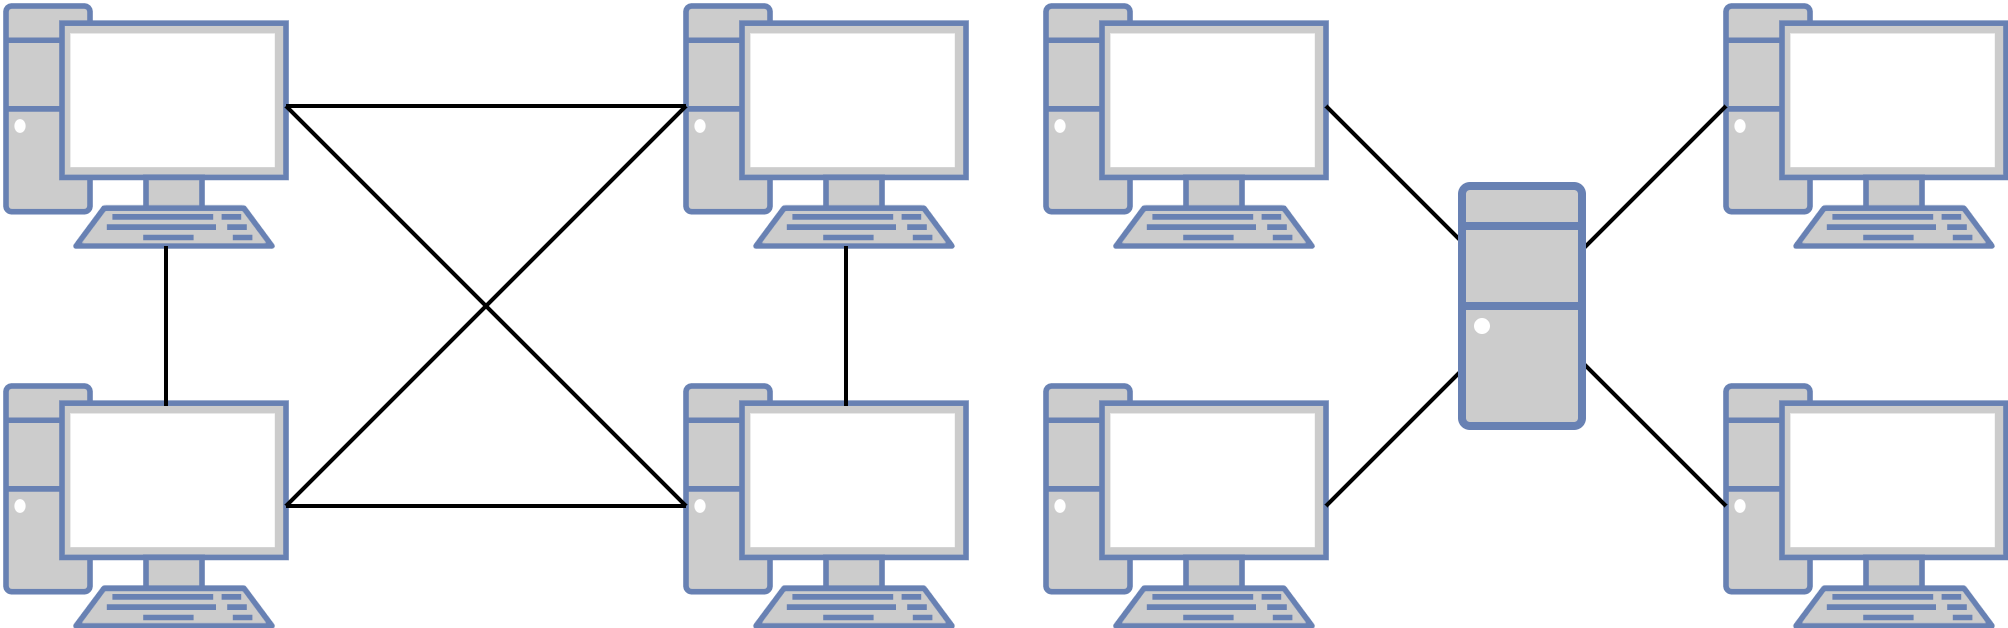
\includegraphics[scale=0.7]{images/Figure2.png}
	\end{center}
	\vspace{-0.6cm}
	\caption{P2P network and client-server network.}
	\label{fig:fig2}
\end{figure}

Peers are creating a sense of virtual community. This community of peers can resolve a greater tasks, beyond those that individual peers can do. Yet, these tasks are beneficial to all the peers in the system~\cite{BandaraJ13}. When request come to such network, node that accepted request is usually called \textbf{coordinator}, because he then is trying to found the right peer to send request to.

Based on how the nodes are linked to each other within the overlay network, and how resources are indexed and located, we can classify networks as~\cite{KamelSE07}:

\begin{itemize}
	\item \textbf{Unstructured} do not have a particular structure by design, but they are formed by nodes that randomly form connections~\cite{FilaliBHB11}. Their strenght and weaknes at the same time is ther lack of structure. These networks and robust when peers join and leave network. But when doing query, they must found more possible peers that have same peace of data. Tipical example of this group is a Gossip-based protocols like~\cite{DasGM02}.
	\item \textbf{Structured} peers are organized into a specific topology, and the protocol ensures that any node can efficiently search the network for a resource. The famos type of structured P2P network is a Distributed Hash Table (DHT). These networks maintain lists of neighbors to do more efficent lookup, and as such they are not so robust when nodes join or leave the network. DHT commonly used in resource loopkup systems~\cite{StoicaMKKB01}, and as efficent resource lookip management and scheduling of applications, or as an integral part of distributed storage systems and NoSQL\cite{Leavitt10} databases.
	\item \textbf{Hybrid} combine previous two models in various ways.
\end{itemize}

P2P networks are great tool in many arsenals, but because their unique ability to act as a server and as a client at the same time we must be aware and pay more attention to security because they are more vulnerable to exploits~\cite{0024003}.
%
%
\subsection{Master-slave}\label{sec:master_slave}
%
In the master-slave architecture, there is one node that is in charge -- \textbf{master}. This node accespt requests, and we usually do not communicate to rest of nodes or \textbf{slaves}. Master node is usually better and more expensive or even specialized hardware such as RAID drives to lower the crush probability. The cluster can also be configured with a \textbf{standby} master, and this node is continually updated from the master node.

But no metter how specialized hardware master runs on, it is prone to fail for varios reasons, so he is a \textbf{single point of failure}. If crush happend, than standby master could continue to server as a master, or new \textbf{leader election} protocol~\cite{KorachKM90} is initiated to pick new master node. 

Master node is responsible for processing any updates to that data. If the master fails, than  the slaves can still handle \textbf{read} requests. Failure of the standby master node, to take over from the master node is a real problem if we want to achieve high-availability system.

Figure~\ref{fig:fig16} show difference between mater-slave $(left)$ and peer-to-peer $(right)$ request handling.

\begin{figure}[H]
	\begin{center}
		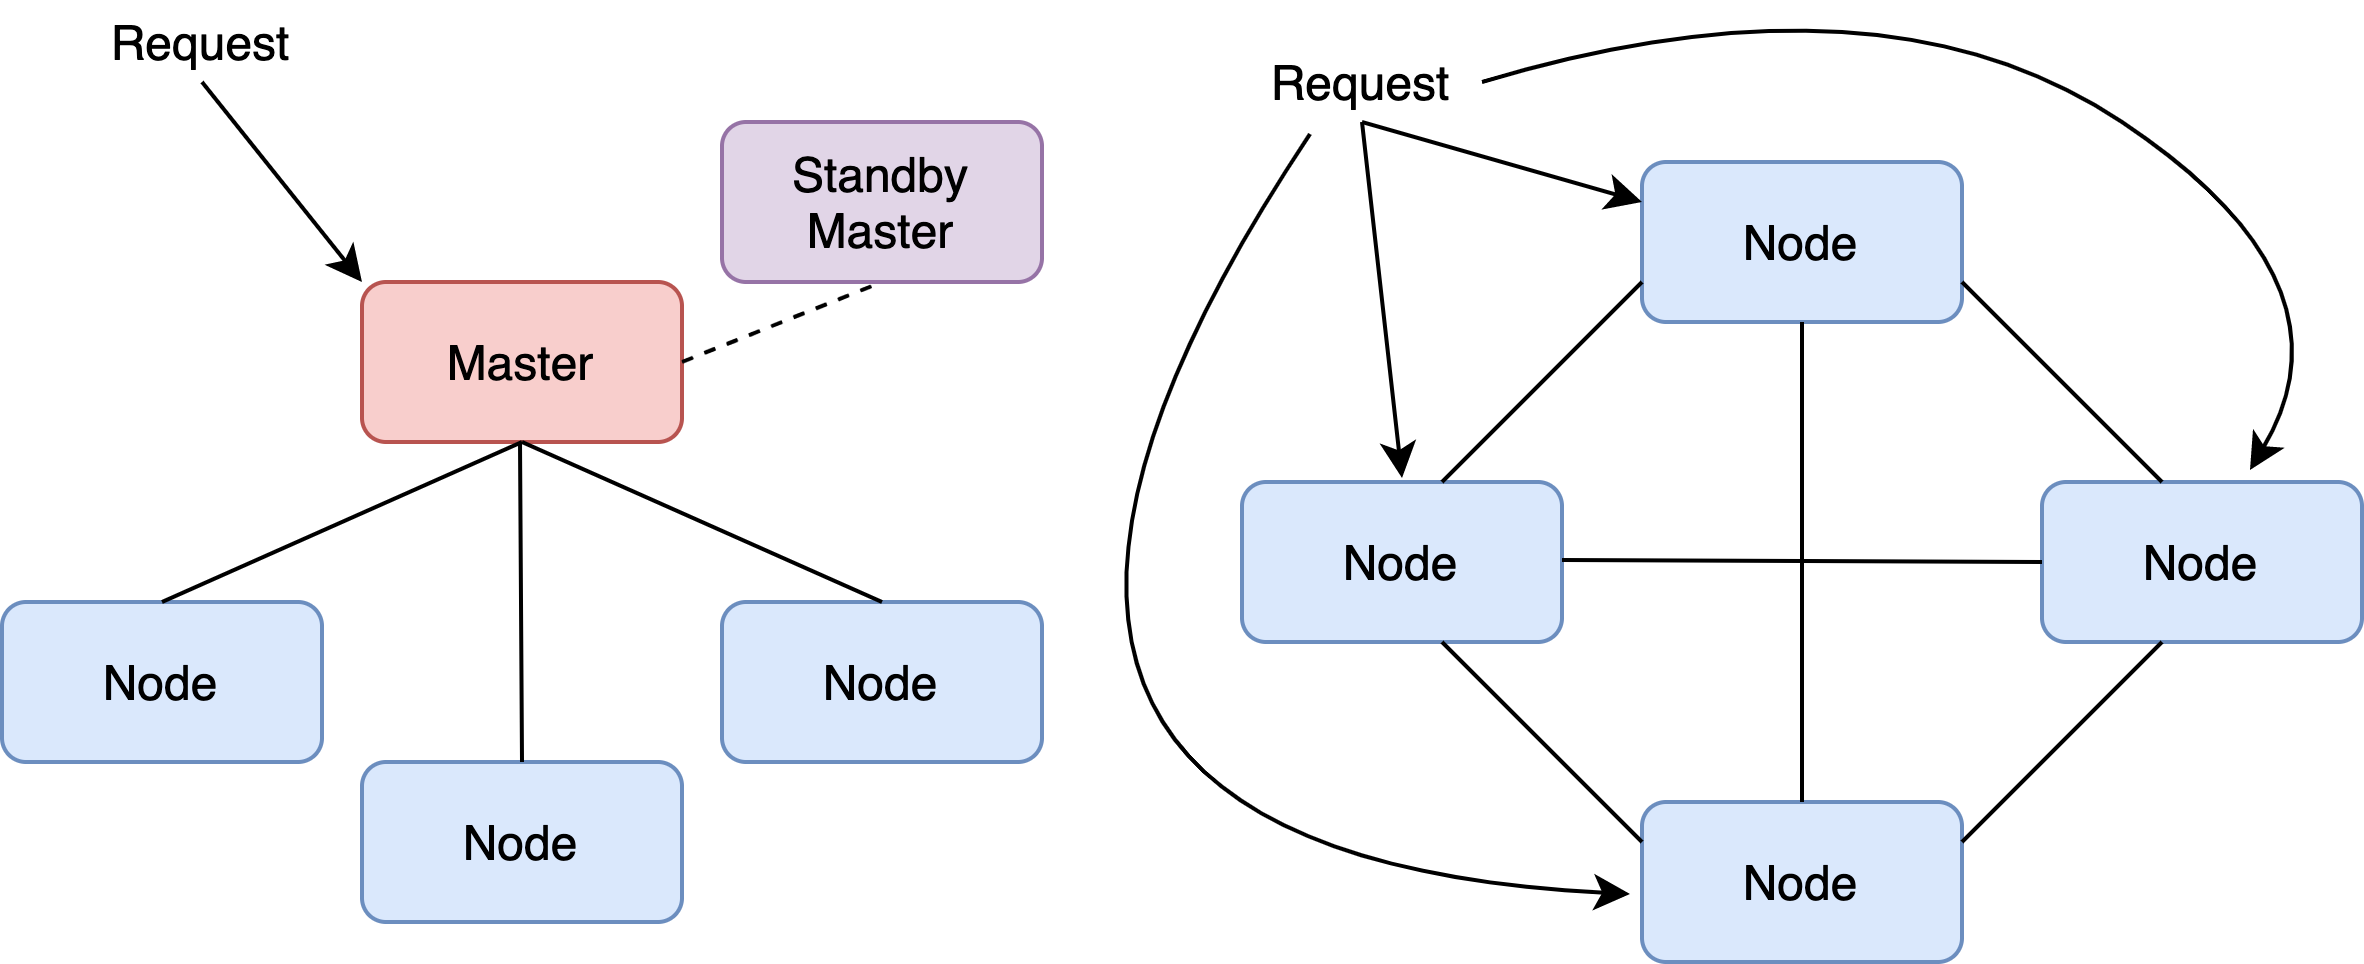
\includegraphics[scale=0.7]{images/Figure16.png}
	\end{center}
	\vspace{-0.6cm}
	\caption{Handling requests master-slave and peer-to-peer}
	\label{fig:fig16}
\end{figure}

Using the right distribution model usually depends on the business requirements. High availability requires a P2P network because no single point of failure. If we could manage data using batch jobs that run in off hours, then the simpler master-slave model might be the solution.
%
%
\section{Similar computing models}\label{sec:similar_models}
%
In this section we are going to shortly describe models that are similar to the DS, and as such they may be the source of confusion.
%
%
\subsection{Parallel computing}\label{sec:parallel_computing}
%
DC and parallel computing seems like models that are the same, and that may share some features like simultaneously executing a set of computations in parallel. Broadly speaking, this is not far from the truth~\cite{Vera16}. 

Distinguished between the two can be presented as follows: in parallel computing all processor units have acces to the shared memory and have some way of the faster inter-process communication, while in DS and DC all processors have their own memory on their own machine and communicate over network to other nodes which is significantly slower. 

These models are similar, but they are not indentical, and the kind of problems they are designed to work on are different. Figure~\ref{fig:fig4} visually summarize the architectural  differences between DC $(up)$ and parallel computing $(down)$.

\begin{figure}[H]
	\begin{center}
		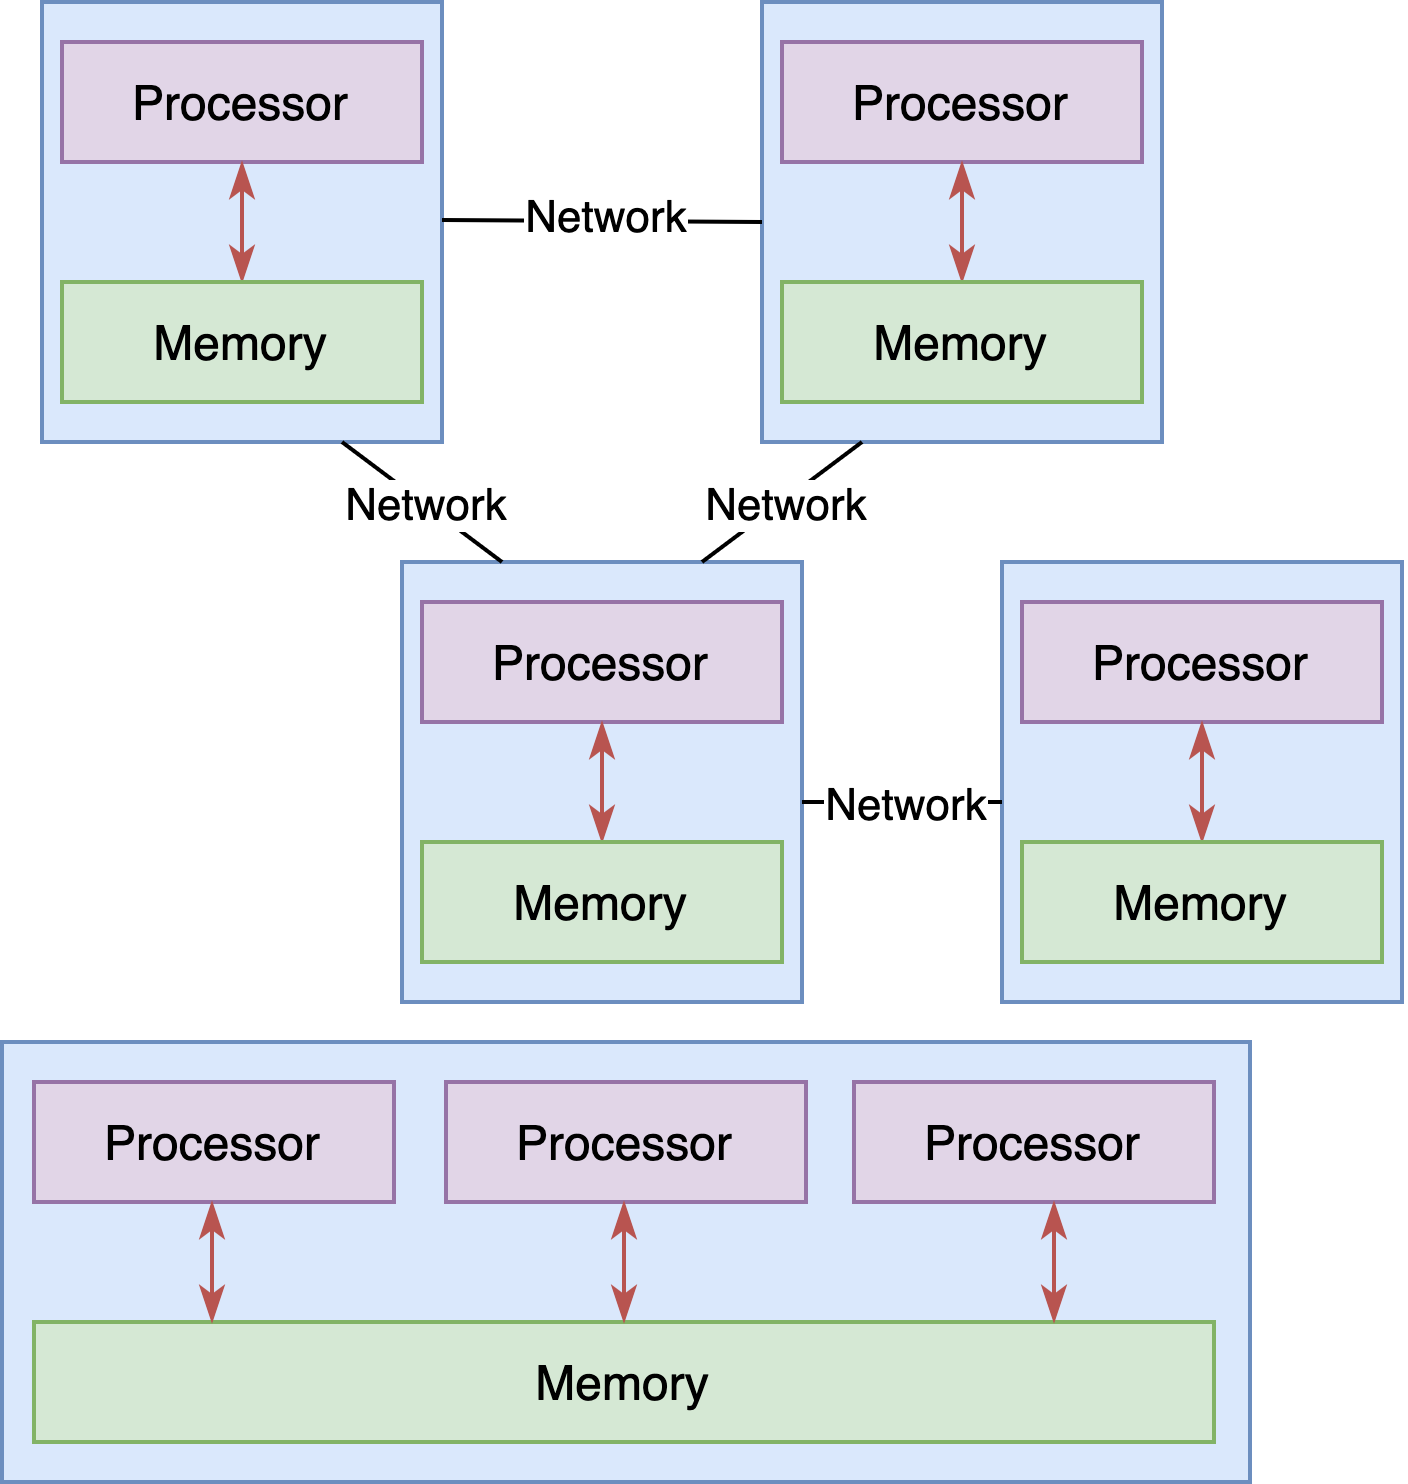
\includegraphics[scale=0.8]{images/Figure4.png}
	\end{center}
	\vspace{-0.6cm}
	\caption{Architectural difference between DC and parallel computing.}
	\label{fig:fig4}
\end{figure}

Parallel computing is often used strategy with problems, that due to their nature or constraints must be done on multi-core machines simultaneously~\cite{0072397}. It is ofthen, that huge problems are divided into smaller ones, which can then be solved at the same time. 

There are number of tasks that requre parallel computing like simulations, computer graphics rendering or different scenarios in scientific computing.
%
%
\subsection{Decentralized systems}\label{sec:decentralized_systems}
%
Decentralized systems are similar to DS, in technical sense they are still DS. But if we take closer look, these systems \textbf{should not} be owned by the single entity. CC for example is perfect example of DS, but it is not decentralized by it's nature. It is centralized systems by the owner like AWS, Google, Microsoft or some other private compay because all computation needs to be moved to big DCs~\cite{HossainRH18}.

By today standards, when we are talking about decentralyzed systems, we usually think of blockchain or blockchain-like technology~\cite{LeibleSSG19}. Since here we have distributed nodes, that are scattered and there is no single entity that own all these nodes. But even if this technology is run in the cloud, it is loosing the decentralized feature. This is the caveat we needs to be aware of. These systems are facing different issues, because any participent in the system might be malicious and they need to handle this case. 

Nontheless, CC can and should be decentralized in a sense that some computation can happend outside of cloud big DCs, closer to the sources of data. These computation could be owned by someone else, and big cloud companies could give their own solution to this as well to relax centralization and problems that CC will have esspecially with ever growing IoT and mobile devices.
%
%
\section{Virtualization techniques}\label{sec:virtualization_techniques}
%
Virtualization as a technique started long ago in time-sharing systems, to provide isolation between multiple users shareing a single system liek a mainframe computer~\cite{CrosbyB06}. 

In~\cite{Sharma} Sharma et al. describe virtualization as technologies which provide a layer of abstraction of the physical computing resources between computer hardware systems and the software systems running on them.

Modeern virtualization diferentiate few different tools. Some of them are used as an integral part of the infrastructure for some flavors like IaaS, while others are used in different CC flavors as well as microservices packageing and distribution format, or are new and still are looking for their place. These options are:

\begin{itemize}
	\item \textbf{Virtual machines (VM)} are the oldest tehnology of the three. In~\cite{Sharma} Sharma et al. describe them as a self-contained operating environment consisting of guest operating system and associated applications, but independent of host operating system. VMs enable us to pack isolation and better utilization of hardware in big DCs. They are vidly used in IaaS environment~\cite{AbsalomBJ13, YangHCLW13} as a base where users can install theirown operating system (OS) and required software tools and applications.
	\item \textbf{Containers} provide almost same functionality to VMs, but there are several subtle differences that make them a goto tool in modern develpment. Instead of the guest OS running on top of host OS, containers use tools that are in Linux kernles like \textit{cgroups} that limits process resource usage so that single process can not starve other processes and use all the resources for himself, and \textit{namespaces} to provide isolation and partitions kernel resources so that single process see node resources like he only exists there. Containers reduce time and footprint from development to testing to production, and they utilize even more hardware resources compared to VMs and show better performance compared to the VMs~\cite{Seo2014PerformanceCA, FelterFRR15}. Containers provide easier way to pack servies and deploy and they are esspecially used in microservices architecture and service orchestration tools like Kubernetes~\cite{BurnsGOBW16}. Google stated few times in their on-line talks that hey have used container technology for all their services, even they run VMs inside containers for their cloud platform. Even though they exist for a while, containers get popularized when companies like Docker and CoreOS developed user-friendly APIs.
	\item \textbf{Unikernels} are the newest addition to the virtualization space. In~\cite{pavlicek2016unikernels} Pavlicek define unikernels as small, fast, secure virtual machines that lack operating systems. Unikernels are comprised of source code, along with only the required system calls and drivers. Because of their specific design, they have single process and they contains and executes what it absolutely needs to nothing more and nothing less~\cite{GoethalsSAVT18}. They are advertised that new technology that will safe resources and that they are \textit{green}~\cite{208735} meaning they save both power and money. When put to the test and compared to containers they give interesting results~\cite{GoethalsSAVT18, PlauthFP17}. Unikernels are still new technology and they are not widly adopted yet. But they give promessing features for the future, esspecially \textbf{if} properly ported to ARM architectures, and various development languages. Unikernes will probably be used as a user applications and functions virtualization tool, because their specific architecture, esspecailly for serverless applications presened in~\ref{sec:microservices}.
\end{itemize}

Figure~\ref{fig:fig5} represent architectural differences between VMs, containers and unikernels.

With every virtualization technique, ultimate goal is to pack as much applications on existing hardware as possible, so that there is no resources that are left not used --- we are trying to achieve high resource utilization.

\begin{figure}[H]
	\begin{center}
		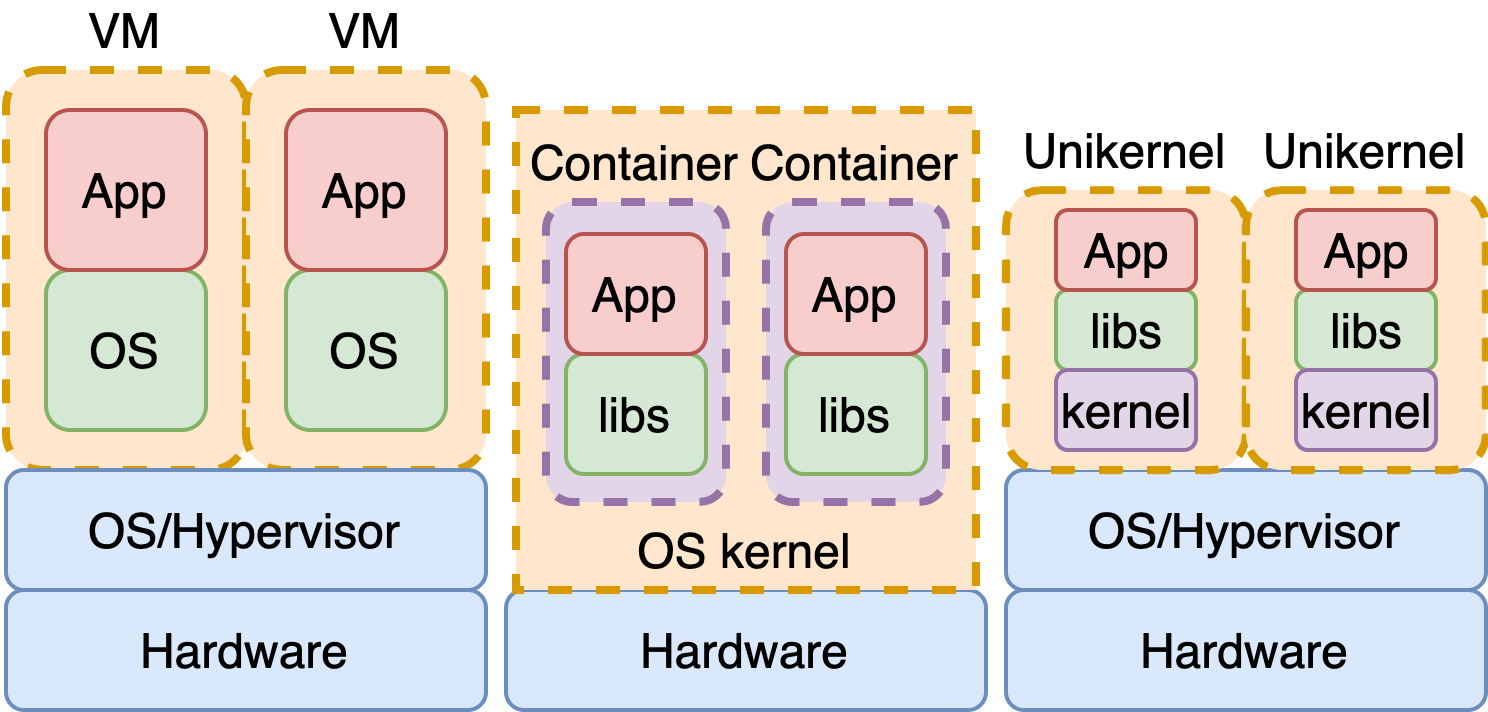
\includegraphics[scale=0.9]{images/Figure5.png}
	\end{center}
	\vspace{-0.6cm}
	\caption{Architectural differences between VMs, containers and unikernels.}
	\label{fig:fig5}
\end{figure}
%
%
\section{Deployment}\label{sec:deployment}
%
Over the years two different approuches evolved how to deploy infrastructure and applications. The difference just get more amplified, when CC and microservices get into the picture, where frequent deployment is very common. 

Here evolve new strategy to mange and deploy complicated infrastructure elements --- Infrastructure as code (IaC). In his book~\cite{wittig2018amazon} Wittig et al. describe it as a process of managing and provisioning computer data centers through machine-readable definition files, rather than physical hardware configuration or interactive configuration tools.

Deplyments in such complex environment can be separated how they handle changes on existing infrastructure or applications on:

\begin{itemize}
	\item \textbf{Mutable model}, is model where we have in place changes which mean that the parts of the existing infrastructure or applications get updated or changed in order to do update. In place change can produce few problems: $(1)$ more risk, beacause in place change my not finish completly which put our infrastructure or the application in possible bad state. This is esspecially probem, if we have a lot of services and multiple copies of the same service. Possibility that our system is not on, is a lot higher, $(2)$ high complexity, this is direct implicatoin of previous feature. Since out change might not get fully done, we can't give guarantis that our infrastructure or applicatoin is transitioned from one version to the another --- change is not \textbf{descrete}, but \textbf{continues} since we might end up in some state in between where we are now and where we want to be.
	\item \textbf{Immutable model}, is model where we do not do any in place changes on existing infrastructure or application whatsoever. In this model, we replace it complety with new version that is updated or changed compared to previous version. Previous version get discarded in favour of new version. Compared to the previous model, immutable deployment have: $(1)$ less risk, since we do not change existing infrastructure or the applicatoin but we start new one with and shut down previous one. This is important esspecially in DS where everyting can fail at any tome, $(2)$ previous property reduce complexity of mutable deployment model. This is direct implicatoin of previous feature, since we shut down and fully replace previous version with new one we get \textbf{descrete} version change and atomic deployment with dafer deployments with fast rollback and recovery processes. On the other hand, this process requre more resources~\ref{Helland16}, since both hersions must be present on the node in order to this process is done. Second problem is data that is used by the app, we should not lost the data that app is generated. If we externalize data than this problems is resolved. We should not rely on local storage, but store that data elsewhere, esspecially when the parts of the system are volatile and changed often. Key adventage of this approuch, is avoiding downtime experienced by the end user when new features are released.
\end{itemize}

Figure~\ref{fig:fig12} summaraze difference bewteen prevous infrastructure deplyment models.

\begin{figure}[H]
	\begin{center}
		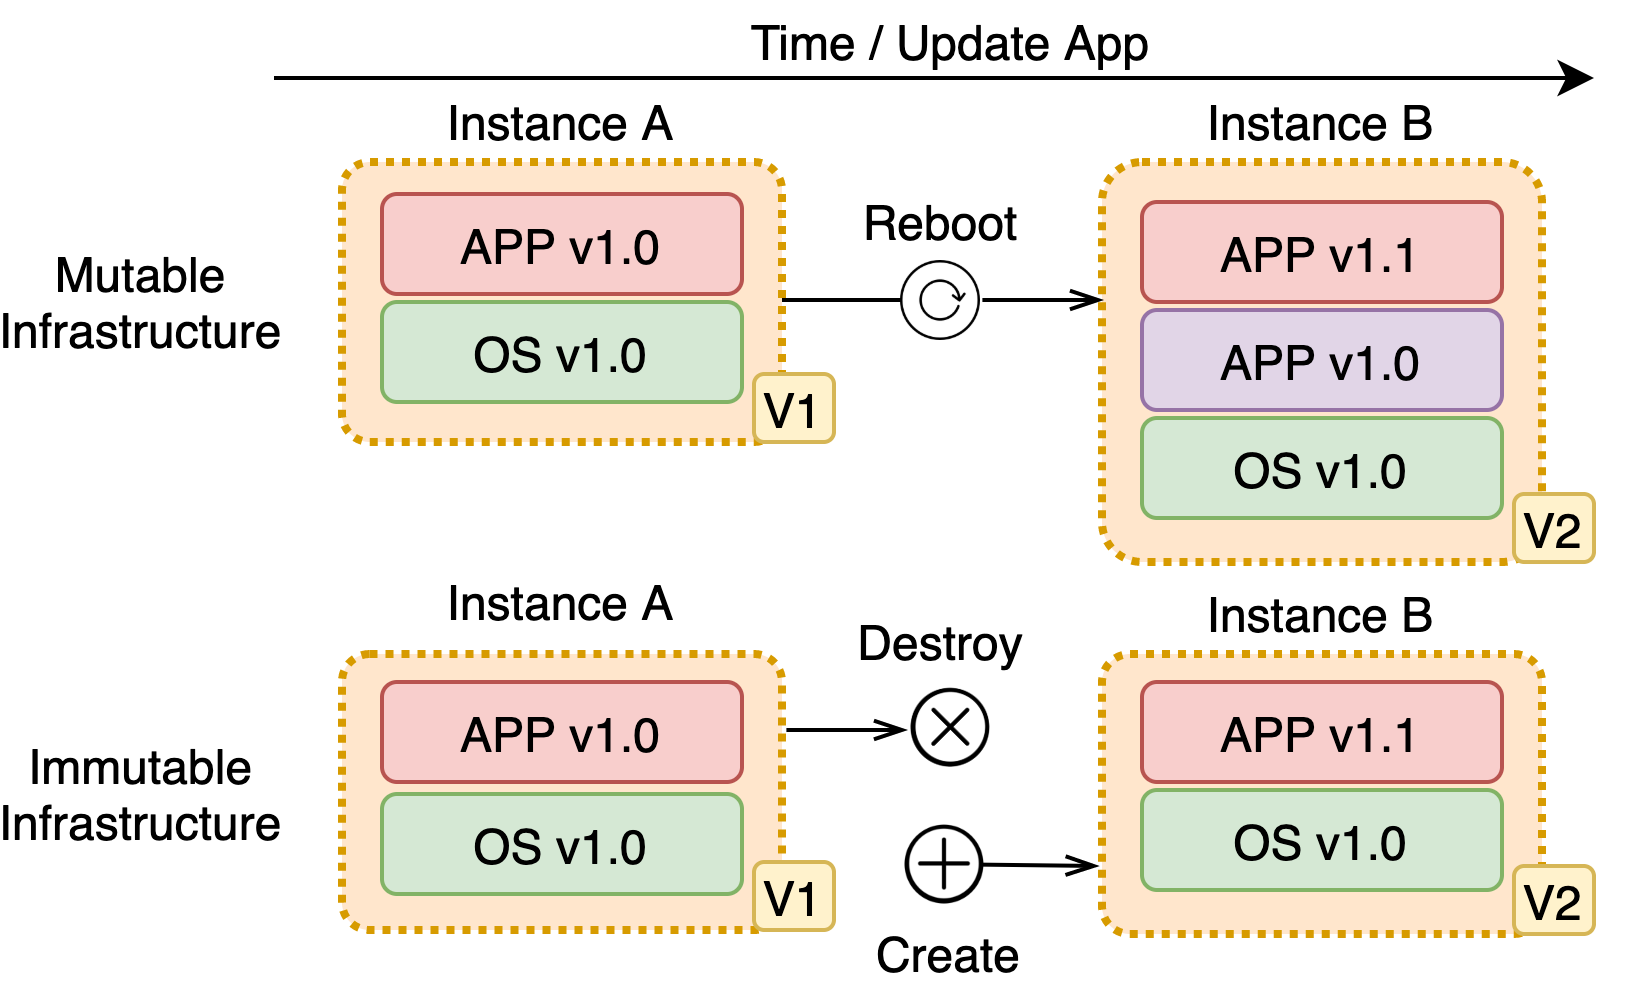
\includegraphics[scale=0.7]{images/Figure12.png}
	\end{center}
	\vspace{-0.6cm}
	\caption{Difference bewteen mutable and immutable deplyment models}
	\label{fig:fig12}
\end{figure}

Immutability is a simple concept to understand, and simplify a lot esspecially in DS~\cite{Helland16}. Write down some data, and ensure that it never changes. It can never be modified, updated, or deleted~\cite{perry2020art}. When this is combined with premisse that we can avoid downtime esspecially in complex DS, it is clear why immutable model is gainign more and more popularity (esspecially with arival of containers). Immutable infrastructure deployment offer few models how to deploy change on the services, even in production to test it, or switch to whole new version. These strategeis include:

\begin{itemize}
	\item \textbf{Blue-Green deployment}, this strategy require two separate environemnts: $(1)$ \textit{Blue} current running version, and $(2)$ \textit{Green} is the new version that needs to be deployed. When we are satisfied that the green version is working properly, we can gradually reroute the traffic from the old environment to the new environment for example by modifying DNS. This strategy offers near zero downtime.
	\item \textbf{Canary update} is the strategy where we do direct a small number of requests to the new version --- the canary. If we are satisfied with the change, we can continue to increase number of requests and monitor how service is working with increasing load, monitor for erros etc.
	\item \textbf{Rolling update} streategy update large environments a few nodes at a time. The setup is similar to blue-green deployment, but here we have single environment. With this strategy, new version gradually replaces the old one. But this is not the only benefit. If for whatever reason, new verrsion is not working properly on larger amount of nodes, we can always do rolling back to previous version.
\end{itemize}

With mutable infrastructure these strategies would be hard to implement, and maybe it is not possible at all. 

Beside infrastructure deployemnt, there is another side that we must consider, and that is how describe these deployments. Here we can consider two different strategies:
\begin{itemize}
	\item \textbf{Imperative}, with this option users have to write code or specific instructions step by step what specific tool need to do in order that application or infrastrucgure is properly setup. In this approuch we have a \textit{smart} user who describe \textit{dumb} machine what is needed to be done and in what order to achieve desired state.
	\item \textbf{Declarative}, with this option user have to describe end state or what is his desired state, and tool needs to figure out the way how to do this. Here we have \textit{smart} system that will found a way how to achieve desired state, and we have user who\textit{do not care} in what order actions need to be done --- that is what system needs to do. User do not need to worry about timing, this simplify whole process and code always represents the latest state. With this type of deployment, we can offer users two different models: $(1)$ use existing formats that are user familiar with like JSON, YAML, XML etc., or $(2)$ create new domain specific language that users need to learn, but we might be able to optimaze description.
\end{itemize}

With introduction of \textit{LinuxKit}, we can create Linux subsystems based around containers, that  are very secure. With linuxkit, every purt of the Linux subsystem is running inside container, so we can assemble a Linux subsystem with services that are needed. As a result, systems created with LinuxKit have a smaller attack surface~\cite{abs-1802-10375} than general purpose systems. This is important from security point of view, but also from infrastructure deployment because we can compose specific OS based around containers that we need for different purpose. And we can update, change and adopt these OS for every machine or purpose we need.

Deployment is based around changeint parts of the OS, and his services that are running inside containers. As a result, everything can be removed or replaced. It's highly portable and can work on desktops, servers, IoT, mainframes, bare metal, and virtualized systems.
%
%
\section{Concurency and parallelism}\label{sec:concurency_parallelism}
%
People usually confuse these two concepts. Even they looks similar, they are different way of doing things. In his talk Rob Pike~\cite{Pike} give great explanation and examples on this topic. In this toke he give great deffinitions of these concepts like:

\begin{itemize}
	\item \textbf{Concurrency} is composition of independently executing things. Concurrency is about dealing with a lot of things at once.
	\item \textbf{Parallelism} is simultaneous execution of multiple things. Parallelism is about doing a lot of things at once. 
\end{itemize}

These things are important, esspecially when building applications and systems that should achieve very high throughput. We must build them with a good structure and a good concurrency model. These features enables possible parallelism, but with communication~\cite{Pike}. These ideas are based on Tony Hoare work of Communicating Sequential Processes (CSP)~\cite{Hoare78}.

\subsection{Actor model}\label{sec:actor_model}
%
In actor model, the main idea is based around \textbf{actors} which are small concurrent code, that communicate independently by sending messages, removing the need for lock-based synchronization~\cite{Hewitt}. This model propose similar idea like Tony Hoare in his work with CSP~\cite{Hoare78}, and actors are oftten confused with CSP. Table~\ref{tab:table6} give differences between actor model and CSP.

\begin{table}[h!]
	\begin{center}
		\begin{tabular}{l|l|l}
			\textbf{Feature} & \textbf{CSP} & \textbf{Actor model}\\
			\hline
			\textbf{Fault tolerance} & Distributed Queue & Hierarchy of supervisors \\
			\textbf{Process identity} & Anonymus & Concrete \\
			\textbf{Composition} & NA & Applicable \\
			\textbf{Communication} & Queue & Direct \\
			\textbf{Message passing} & Sync & Async\\
		\end{tabular}
	\end{center}
	\vspace{-0.5cm}
	\caption{Ddifferences between actor model and CSP.}
	\label{tab:table6}
\end{table}

Actors do not share memory, and they are isolated by nature. Actor can create another actor/s and even watch on them in case they stop unexpectedly. And when an actor finished its job, and he is not needed anymore, it disappears. These actors can create complicated networks that are easy to understand, model and reason about and everything is based on a simple massage passing mechanism. 

Every actor have a designated message box. When a message arrives, actor will test message type and do job acording to message type he received. In this way we are not dependent of lock-based synchronization that can be hard to understand, and it can cause serious problems.

Actor model is fault tolerant by design. It support crush to happend, because there is a \say{self heal} mechanism that will monitor actor/s, and when crash happend it will try to apply some strategy, in most cases just restart actor, but other strategies could be applied. This philosophy is really usefull, because it is hard to think about every single failure option.
%
%
\section{Motivation and Problem Statement}\label{sec:problem_statement}
%
In~\cite{GreenbergHMP09} Greenberg et al. point out that micro data-centers (MDCs) are used primarily as nodes in content distribution networks and other \say{embarrassingly distributed} applications.

One size never fits all, so the cloud should not be our final computing shift. Various models presented in~\ref{sec:mobile_computing}, show possibility that computing could be done closer to the data source, to lower the latency for its clients by contacting the cloud only when needed, while heavy computation remains in the cloud because of resource availability. Send to the cloud only information that is crucial for other services or applications~\cite{inproceedingsSimic1}. Not ingest everything as the standard cloud model proposes.

MDCs with a zone-based server organization is a good starting point for building EC as a service, but we need a more available and resilient system with less latency. EC originates from P2P systems~\cite{LopezMEDHIBFR15} as sugested by L{\'{o}}pez et al., but expands it into new directions and blends it with the CC. But, infrastructure deployment will not happen until the process is trivial~\cite{SatyanarayananBCD09}. Going to every node is tedious and time consuming. Especially when geo-distribution is taken into consideration.

A well defined system could be offered as a service, like any other resource in the CC. We can offer it to researchers and developers to create new human-centered applications. If we need more resources on one side, we can take from one pool of resources and move to another one.
But on the other hand, some CC providers might choose to embed it into their own existing system, hiding unnecessary complexity, behind some communication interface or proposed application model.

The idea of small servers with heterogeneous compute, storage, and network resources, raise interesting research idea and motivation for this thesis. Taking advantage of resources organized locally as micro clouds, community clouds, or edge clouds~\cite{RydenOCW14} suggested by Ryden et al., to help power-hungry servers reduce traffic~\cite{HirschMZ18}. Contact the cloud only when needed~\cite{inproceedingsSimic1}. Send to the cloud only information that is crucial for other services or applications. Not ingest everything as the standard CC model proposes.

To achieve such behavior, dynamic resource management, and device management is essential. We must perceive available resources, configuration, and utilization~\cite{GubbiBMP13, WangZZWYW17}. Traditional DCs is a well organized and connected system. On the other hand, these MDCs consist of various devices, including ones presented in~\ref{sec:mobile_computing} that are not~\cite{JiangCGZW19}. This idea, brings us to the problem this thesis address.

EC and MDCs models lack dynamic geo-organization, well defined native applications model, and clear separation of concerns. As such they cannot be offered as a service to the users. They usually exist independently from one another, scattered without communication between them, offered by providers who mostly lock users in their own ecosystem. Co-located edge nodes should be organized locally, making the whole system and applications more available and reliable, but also extending resources beyond the single node or group of nodes, maintaining good performance to build servers and clusters~\cite{ArocaG12}.

This cloud extension deepens and strengthens our understanding of the CC as a whole. With the separation of concerns setup, EC native applications model, and a unified node organization, we are moving towards the idea of EC as a service. 

Based on this, we define the problem through the following research questions three segments:

\begin{enumerate}[start=1,label={(\bfseries \arabic*)}]
	\item \textit{Can we organize geo-distributed edge nodes in a similar way to the cloud, adopted for the different  environment, with clear separation of concerns and familiar applications model for users.}
	\item \textit{Can we offer these organized nodes as a service to the developers and researchers for new human-centered applications, based on the cloud pay as you go model?}
	\item \textit{Can we make model in such a way that is formaly correct, easy to extend, understand and reason about?}
\end{enumerate}

This cloud-like extension makes the whole system and applications more available and reliable, but also extends resources beyond the single node. Satyanarayanan et al. in ~\cite{SatyanarayananK19} show that MDCs can serve as firewalls, while Simi\' c et al., in~\cite{inproceedingsSimic1} use similar idea as pre-processing tier. At the same time, users are getting a unique ability to dynamically and selectively control the information sent to the cloud. Years after its inception, EC is no longer just an idea~\cite{SatyanarayananK19} but a must-have tool for novel applications to come.
%
%
\section{Research Hypotheses, and Goals}\label{sec:research_hyphotesis_and_golas}
%
Based on reserach questions and motivation presented in~\ref{sec:problem_statement}, we derive the hypotheses around which the thesis is based. It can be summarized as follows:

\begin{enumerate}[start=1,label={(\bfseries \arabic*)}]
	\item \textbf{Hypothesis:} \textit{It is possible to organize EC nodes in a standard way based on cloud architecture, with adaptation for an EC geo-distributed environment. Give users the ability to organize nodes in the best possible way in some geographic areas to serve only the local population in near proximity.}
	\item \textbf{Hypothesis:} \textit{It is possible to offer it to researchers and developers to create new human-centered applications. If we need more resources on one side, we can take from one pool of resources and move to another one, or organize them any other way needed.}
	\item \textbf{Hypothesis:} \textit{It is possible to present clear separation of concerns for the future EC as a service model, and establish a well-organized system where every part has an intuitive role.} 
	\item \textbf{Hypothesis:} \textit{It is possible to present unified model that supports heterogeneous EC nodes, with a set of technical requirements that nodes must fulfil, if they want to join the system.}
	\item \textbf{Hypothesis:} \textit{It is possible to present a clear application model so that users can use full potential of newly created infrastructure.}
\end{enumerate}

From the previously defined hypotheses, we can derive the primary goals of this thesis, where the expected results include:

\begin{enumerate}[start=1,label={(\bfseries \arabic*)}]
	\item \textit{The construction of a model with a clear separation of concerns for the model influenced by cloud organization, with adaptations for a different environment. With a model for EC applications utilizing these adaptations. This addresses the first research question, and is the topic of Chapter~\ref{chapter:Micro_clouds}.}
	\item \textit{The constructed model is more available, resilient with less latency, and as such it can be offered to the general public as a service like any other service in the cloud. This addresses the second research question, and is the topic of Chapter~\ref{chapter:Micro_clouds}.}
	\item \textit{The constructed model is described formaly well, using solid mathematical theory, but also easy to extend both formaly and technicaly, easy to understand and reason about. This addresses the third research question, and is the topic of Chapter~\ref{chapter:Micro_clouds}.}
\end{enumerate}
%
%
\section{Structure of the thesis}\label{sec:structure_of_thesis}
%
Throughout this introductory Chapter, we defined the motication for out work with problems that this thesis addresses and presented the necessary background informations and areas to support our work. Here we outline the rest of the thesis.

Chapter~\ref{chapter:Review} presents the literature review, where we examine different aspects of existing systems and methods important for the thesis. We analyze existing nodes organizational abilities in both industry and academia frameworks and solutions to address our first research question. We further exemine platform models from industry and academia tools and frameworks to address our second research question. And last but not least, we examine current strategies to offload tasks from the cloud. All three parts address our third research question.

Chapter~\ref{chapter:Micro_clouds} details our model, how it is related to other research and where it connects to other existing models and solutions. We further describe our solution as well as protocols requried for such sysrtem to be implemented foramly. We give examples of how exisintg infrastructure could be used, as well as familiar application model for developers. 

Chapter~\ref{chapter:Implementation} present implementation details of an framework developed to test hypotheses defined earlier in this chapter, but also model and foramly defined protocols defined in~\ref{chapter:Micro_clouds}. This chapter also show results after conducting experiments, current limitations of implemented system, and possible applications that could benefit from such system.

Chapter~\ref{chapter:Conclusion} concludes our work and presents opportunities for further research and development.
%
%